% % % % % % % % % % % % % % % % % % % % % % % % % % % % % % % % % % % % % % % %
% LaTeX4EI Template for Cheat Sheets                                Version 1.0
%
% Authors: Emanuel Regnath, Martin Zellner
% Contact: info@latex4ei.de
% Encode: UTF-8, tabwidth = 4, newline = LF
% % % % % % % % % % % % % % % % % % % % % % % % % % % % % % % % % % % % % % % %


% ======================================================================
% Document Settings
% ======================================================================

% possible options: color/nocolor, english/german, threecolumn
% defaults: color, english
\documentclass[english]{latex4ei/latex4ei_sheet}

% set document information
\title{Signal Processing and\\ Machine Learning}
\author{LaTeX4EI}					% optional, delete if unchanged
\myemail{info@latex4ei.de}			% optional, delete if unchanged
\mywebsite{www.latex4ei.de}			% optional, delete if unchanged


%\DeclareMathOperator{\T}{\textsf{\textit{T}}}		% Zufallsvariable X
\DeclareMathOperator{\Bias}{Bias}		% Zufallsvariable X
\DeclareMathOperator{\argmax}{argmax}

\DeclareMathOperator{\rang}{rang}
\renewcommand{\vec}[1]{\underline{\boldsymbol{#1}}}
%\renewcommand{\vec}[1]{\boldsymbol{#1}}



\newcommand{\x}{\textit{x}}
\newcommand{\vx}{\underline{\textbf{\textit{x}}}}
\newcommand{\VX}{\underline{\textbf{\textit{X}}}}

\newcommand{\y}{\textit{y}}
\newcommand{\vy}{\underline{\textbf{\textit{y}}}}
\newcommand{\VY}{\underline{\textbf{\textit{Y}}}}


\newcommand{\VA}{\underline{\textit{A}}}
\newcommand{\A}{\textit{A}}
\newcommand{\va}{\underline{\textbf{\textit{a}}}}

\newcommand{\VB}{\underline{\textit{B}}}




% ======================================================================
% Begin
% ======================================================================
\begin{document}

\IfFileExists{git.id}{\input{git.id}}{}
\ifdefined\GitRevision\mydate{\GitNiceDate\ (git \GitRevision)}\fi
% Title
% ----------------------------------------------------------------------
\maketitle   % requires ./img/Logo.pdf



% Section
% ----------------------------------------------------------------------
\section{Statistical Learning}
% ======================================================================

\begin{sectionbox}
	\subsection{Definition}
	\textbf{Statistical Model}
	\begin{tablebox}{lll}
		Statistical Model: & $\{\mathbb X, \mathbb F, \P_θ ; θ \in \Theta\}$  \\
		Sample Space: & $Ω$\\
		Observation Space: & $\mathbb X$\\
		Sigma Algebra: & $\mathbb F$ \\
		Probability: & $\P_{\theta}$\\
		Test (decision rule): & $T:\mathbb X \mapsto \{\theta_{0},\theta_{1}\}, x \mapsto T(x)$\\
		Null Hypothesis: & $H_0: \theta \in \Theta_0 $  \\ 
		Alternative Hypothesis: &  $H_1: \theta \in \Theta_1 $\\
	\end{tablebox}
	\textbf{Cost Criterion $G_T$}:\\
	$G_T : \{\theta_0,\theta_1\} \mapsto [0,1], \theta \mapsto P(\{T(X)=1\};\theta)\\=E[T(X);\theta] = \int\limits_{\mathbb{X}}^{}{T(x)f_{X}(x;\theta)\diff x}$\\
	\textbf{Error Level $\alpha$}: $G_T(\theta_0) \leq \alpha$\\
	\textbf{Two Error Types}:\\
	False Alarm: $\theta = \theta_0, T(x)=1\\
	G_T(\theta_0)=P(\{T(X)=1\};\theta_0)$\\
	Detection Error: $\theta = \theta_1, T(x)=0\\
	1-G_T(\theta_1)=P(\{T(X)=0\};\theta_1)$\\
	
\end{sectionbox}

 
\begin{sectionbox}
	\subsection{Maximum Likelihood Test}
	\textbf{ML Ratio Test Statistic}:\\	
	$R(x) = \begin{cases}
		\frac{f_{\X}(x;θ_1)}{f_{\X}(x;θ_0)}&;\quad f_X(x;\theta_0)>0\\
		\quad\quad\infty&;\quad f_X(x;\theta_0)=0$ and $f_X(x;\theta_1)>0
	\end{cases}$\\
	\textbf{ML Test}:\\	
	$T_{\ir ML} : \mathbb{X} \mapsto \{0,1\}, x\mapsto \begin{cases}
		1&;\quad R(X)>c\\
		0&;\quad$ otherwise
	$\end{cases}$\\
	if $c \ne 1$ False Alarm Error Probability can be adjusted $\rightarrow$ Neyman Pearson Test
\end{sectionbox}

\begin{sectionbox}
	\subsection{Neyman-Pearson-Test}
	The best test of $\P_0$ against $\P_1$\\
	%NP-Test to the level $\alpha$:
	%$c$ is chosen as: $c = (1-\alpha)-quantile of f_x(x;\theta_0)$
	\parbox{15em}{$T_{\ir NP}(x) = \begin{cases} 1 & R(x) > c\\ γ & R(x) = c \\ 0 & R(x) < c \end{cases}$} \quad \parbox{15em}{ Likelihood-Ratio: \\ $R(x) = \frac{f_{\X}(x; θ_1)}{f_{\X}(x; θ_0)}$ }\\
	$γ = \frac{α - \P_0(\{R > c\})}{\P_0(\{R = c\})}$ \quad Errorlevel $α$\\
	Steps: For $α$ calculate $x_{α}$, then $c = R(x_{α})$\\
	\\
	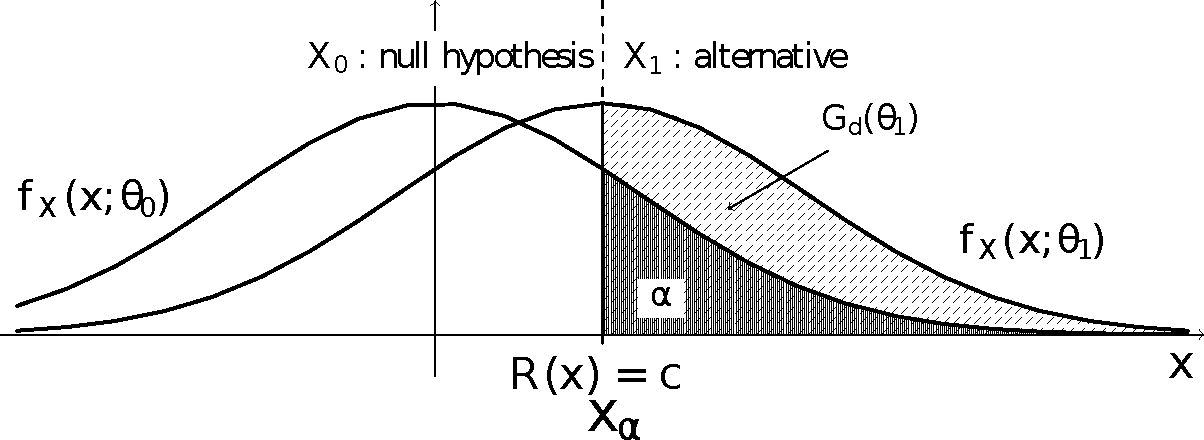
\includegraphics[width = \columnwidth]{tests}
	
	\textbf{Maximum Likelihood Detector:} \quad
	$T_{\ir ML}(x) = \begin{cases} 1 & R(x) > 1 \\ 0 & \text{otherwise} \end{cases}$\\
	\textbf{ROC Graphs:} plot $G_T(θ_1)$ as a function of $G_T(θ_0)$
\end{sectionbox}

\begin{sectionbox}
	\subsection{Bayes Test (MAP Test)}
	Prior knowledge about possible hypotheses:\\$\P(\{θ ∈ Θ_0 \}) + \P(\{θ ∈ Θ_1\}) =  1 $\\ 
	$T_{\ir Bayes} = \underset{T}{\operatorname{argmin}}\{P_{\epsilon}\}= 
	\begin{cases} 1 &;\quad\!\frac{f_{X}(x|θ_1)}{f_{X}(x|θ_0)} > c\\
	0&;\quad\text{otherwise}\end{cases} \\= \begin{cases} 1&;\quad \P(θ_1|x) > \P(θ_0|x) \\ 0 &;\quad \text{otherwise} \end{cases}\\
	\text{with}:\\ 
	P_{\epsilon} = P(\theta_0)G_T(\theta_0)+P(\theta_1)(1-G_T(\theta_1)),\quad c = \frac{P(\theta_0)}{P(\theta_1)}$\\\\
	\textbf{if} $P(\theta_0) = P(\theta_1) \implies T_{\ir Bayes} = T_{\ir ML}$\\\\
	\textbf{Multiple Hypothesis} $\{\theta_0,...,\theta_k\}; \mathbb{X}_0,...,\mathbb{X}_k \in \mathbb{X}$:\\
	$T_{\ir Bayes} = \underset{k\in1,...,K}{\operatorname{argmin}}\{P(\theta_k|x)\}$\\\\
	\textbf{Loss Function}:\\
	$L(T(x), θ) = \begin{cases} L_0 &;\quad T(x) = 1, \text{ but }θ = θ_0\quad \text{(FALSE ALARM)} \\
	L_1 &;\quad T(x) = 0, \text{ but }θ = θ_1\quad \text{(DETEC. ERROR)}\\
	0 &;\quad \text{otherwise} \end{cases}$\\
	$L_i$ denotes the Loss Value in cases where the correct decision parameter $θ_i$ is missed.\\
	$\operatorname{Risk}(T) = \E[L(T(\X), θ)] = \E [\E [L(T(x), θ)|x = \X ]]$\\
\end{sectionbox}

\begin{sectionbox}
	\subsection{Linear Alternative Tests}
	
	Estimate normal vector $\vec w^\top$ and $w_0$, which separate $\mathbb X$ into $\mathbb X_0$ and $\mathbb X_1$\\
	$\log R(\vec x) = -\frac{1}{2}\ln(\frac{\det(\ma C_1)}{\det(\ma C_0)}) - \frac{1}{2}(\vec x- \vec{μ}_1)^\top\ma C_1^{-1}(\vec x- \vec{μ}_1) +\\+\frac{1}{2}(\vec x- \vec{μ}_0)^\top\ma C_0^{-1}(\vec x- \vec{μ}_0) = \ln(\frac{P(\theta\in\Theta_0)}{P(\theta\in\Theta_1)})$ (seperating surface)\\\\
	For Gaussian $f_X(x; \mu_k, C_k)$ with $θ_0$ and $θ_1$ corresponding to $\{\mu_0,C_0\}$ and $\{\mu_1, C_1\}$, it follows that
	\begin{itemize}
		\item if $C_0 \ne C_1$, $logR(x) = 0$ is non-linear and the separating surfaces are surfaces of second order:
		parabolic, hyperbolic, or elliptic surfaces.
		\item if $C_0 = C_1$, $logR(x) = 0$ is affine and thus defines a hyperplane in $\mathbb{X}$ which decomposes $\mathbb{X}$ into $\mathbb{X}_0$ and $\mathbb{X}_1$, i.e.,\\
		$T: \mathbb X \ra \R, \vec x \mapsto \begin{cases} 1 & \vec w^\top \vec x > w_0\\ 0 & \text{otherwise}\end{cases}$\\
		\begin{itemize}
			\item case 1: $\ma C_0 = \ma C_1 = \sigma^2\ma I_N$\\
			$\vec w^\top = (\vec\mu_1-\vec\mu_0)^\top,\\
			w_0= \frac{1}{2}(\vec\mu_1^\top\vec\mu_1-\vec\mu_0^\top\vec\mu_0) -\sigma^2\ln(\frac{P(\theta\in\Theta_1)}{P(\theta\in\Theta_0)})$\\
			$\vec w$ colinear with $(\vec \mu_1-\vec \mu_0)\\\implies \text{hyperplane orthogonal to } (\vec \mu_1-\vec \mu_0)$ 
			\item case 2: $\ma C_0 = \ma C_1 = \ma C$\\
			$\vec w^\top = (\vec\mu_1-\vec\mu_0)^\top\ma C^{-1},\\
			w_0= \frac{1}{2}(\vec {μ}_1 - \vec{μ}_0)^\top \ma C^{-1} (\vec {μ}_1 + \vec{μ}_0) -	\ln(\frac{P(\theta\in\Theta_1)}{P(\theta\in\Theta_0)})$\\
			in general $\vec w$ \textbf{not} colinear with $(\vec \mu_1-\vec \mu_0)\\\implies \text{hyperplane \textbf{not} orthogonal to } (\vec \mu_1-\vec \mu_0)$ 
		\end{itemize}
		\item if $C_0 = C_1$ and $\mu_0 = −\mu_1$, $log R(x) = 0$ is linear and defines a separating hyperplane in $\mathbb{X}$ which contains the origin, i.e.,\\
		$T: \mathbb X \ra \R, \vec x \mapsto \begin{cases} 1 & \vec w^\top \vec x > 0\\ 0 & \text{otherwise}\end{cases}$\\
	\end{itemize}
	
	
	% Bild aus Part7 p 197!!!
	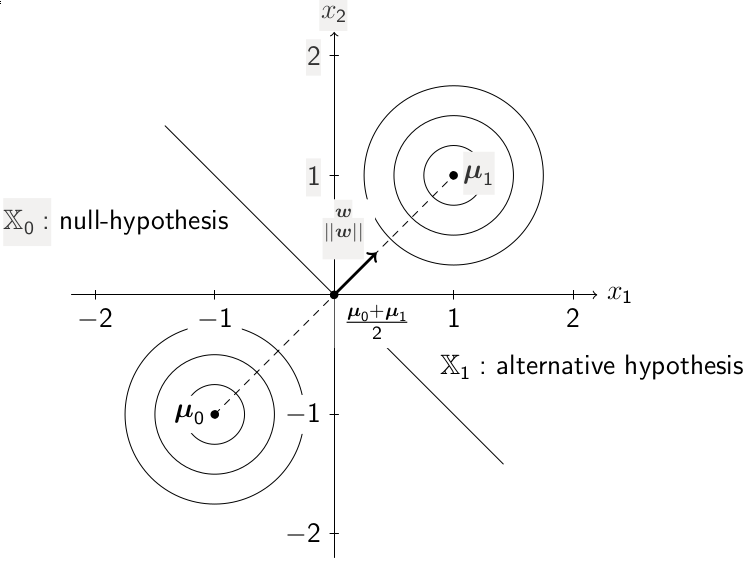
\includegraphics[width = \columnwidth]{linest2}
	
\end{sectionbox}

% Section
% ----------------------------------------------------------------------
\section{Learning and Generalization}

\begin{sectionbox}
	\subsection{Empirical Risk Function and Generalization Error}
	ML scenarios (unknown Stochastical Model) base learning on:
	$Risk_{emp}(T;\mathbb{S})=\frac{1}{M}\sum_{i=1}^{M}L(T(\vx_i),y_i),\quad(\vx_i,y_i)\in\mathbb{S}$
	
	$\vx\mapsto T(\vx;\mathbb{S})\quad T=\underset{T'\in\mathbb{T}}{\operatorname{argmin}}\{Risk_{emp}(T';\mathbb{S})\}$
	
	\textbf{good Generalization}: $Risk_{emp}(T;\mathbb{S}_{test})$ similar to $Risk_{emp}(T;\mathbb{S})$ 
	\textbf{bad Generalization}:
	\begin{itemize}
		\item small $\mathbb{T}$ that does not cover $T_{opt}$ $\rightarrow$ cannot be selected by ML
	\end{itemize}
	$\Rightarrow$ strong mismatch between the desired and derived \textit{Test} and refers to a sort of \textit{Bias Error Term}
	\begin{itemize}
		\item too rich $\mathbb{T}$ $\rightarrow$ fluctuating of the available data (measurement noise) is interpreted as meaningful information
	\end{itemize}
	$\Rightarrow$ \textit{Overfitting}; leads to an increased \textit{Variance Error Term}
	
\end{sectionbox}

\begin{sectionbox}
	\subsection{Bias-Variance Decomposition}
	$Risk=E_{S,X,Y}[L(T(X;S),Y)]=E_X[1-P_{Y|X}(Y=T_B(X))+(1-P_{S|X}(T(X;S)=T_B(X)))(2P_{Y|X}(Y=T_B(X))-1)],\quad T_B(X)$ is the unknown \textit{Bayes Test}
	
	If the potential set $\mathbb{S}$ would be selected from a distribution such that the derived Test $T(\vx; \mathbb{S})$ and the corresponding Bayes Test $T_B(\vx)$ are identical almost surely, then the Risk Function achieves its minimum value which is equal to the \textit{Irreducible Error} $E_X[1 − P_{Y|X}(Y = T_B(X))]$(denotes the probability that for a given input $\vx$ the Bayes Test $T_B(X)$
	decides for the false label $y$).
	
\end{sectionbox}

% Section
% ----------------------------------------------------------------------
\section{Classification Trees and Random Forests}

\begin{sectionbox}
	\subsection{CART Algorithms}
	
\end{sectionbox}

\begin{sectionbox}
	\subsection{Random Forests}	
	
\end{sectionbox}


% Section
% ----------------------------------------------------------------------
\section{Hypothesis Testing}
making a decision based on the observations

\begin{sectionbox}
	\subsection{Definition}

	Null hypothesis $H_0: θ ∈ Θ_0$ (Assumed first to be true)\\
	Alternate hypothesis $H_1: θ ∈ Θ_1$ (The one to proof) \\
	Descision rule $φ: \mathbb X \ra [0, 1]$ with \\
	$φ(x) = 1$: decide for $H_1$, $φ(x) = 0$: decide for $H_0$
	Error level $α$ with $\E[d(\X)|θ] \le α, ∀θ∈Θ_0$

	\begin{tablebox}{p{7mm}llp{17mm}}
		Error Type & ${}_{\text{Decision}}$\!{\large $\diagdown$}\!${}^{\text{Reality}}$ & $H_1$ false {\small ($H_0$ true)} & $H_1$ true {\small ($H_0$ false)}
		\\ \cmrule
		1 (FA) False& $H_1$ rejected & \textbf{T}rue \textbf{N}egative & \textbf{F}alse \textbf{N}egative (Type 2)
		\\
		Alarm & \small ($H_0$ accepted) & $\P = 1-α$  & $\P = β$
		\\[1em]
		2 (DE) & $H_1$ accepted & \textbf{F}alse \textbf{P}ositive (Type 1) & \textbf{T}rue \textbf{P}ositive
		\\
		Detection Error & \small($H_0$ rejected) & $\P = α$ & $\P = 1-β$
	\end{tablebox}
	Power:
	Sensitivity/Recall/Hit Rate: $\frac{\text{TP}}{\text{TP}+\text{FN}}=1-β$\\
	Specificity/True negative rate: $\frac{\text{TN}}{\text{FP}+\text{TN}}=1-α$\\
	Precision/Positive Prediciton rate: $\frac{\text{TP}}{\text{TP}+\text{FP}}$\\
	Accuracy: $\frac{\text{TP} + \text{TN}}{\text{P}+\text{N}} = \frac{2-α-β}{2}$


	\subsubsection{Design of a test}
	Cost criterion $G_{φ}: Θ \ra [0, 1], θ \mapsto \E[d(X)|θ]$\\
	False Positive lower than $α$: $G_d(θ)|_{θ∈Θ_0} ≤ α, ∀ θ ∈ Θ_0$\\
	False Negative small as possible: $\max \{G_d(θ)|_{θ∈Θ_1}\}, ∀ θ ∈ Θ_1$
\end{sectionbox}



\begin{sectionbox}
	\subsection{Sufficient Statistics}
	Sufficiency for a test $T(\X)$ means that no other test statistic, i.e., function of the observations $\vec x$,
contains additional information about the parameter $θ$ to be estimated:\\
$f_{\X|T} (x|T(x) = t, θ) = f_{\X|T}(x|T (x) = t)$

\end{sectionbox}


% Section
% ----------------------------------------------------------------------
\section{Math}
% ======================================================================

\begin{sectionbox}
	\begin{tabular}{@{}llll}
		$\pi \approx \num{3,14159}$ & $e \approx \num{2,71828}$ & $\sqrt{2} \approx \num{1,414}$ & $\sqrt{3} \approx \num{1,732}$ \\
	\end{tabular}

	\textbf{Binome, Trinome}\\
	$(a\pm b)^2 = a^2 \pm 2ab + b^2$ \hfill $a^2 - b^2 = (a-b)(a+b)$\\
	$(a \pm b)^3 = a^3 \pm 3a^2b + 3ab^2 \pm b^3$\\
	$(a+b+c)^2 = a^2 + b^2 + c^2 + 2ab + 2ac + 2bc$
	\\[0.5em]
	\textbf{Folgen und Reihen}\\
	$\underset{\text{Aritmetrische Summenformel}}{\sum \limits_{k=1}^{n} k = \frac{n (n+1)}{2}}$ \quad $\underset{\text{Geometrische Summenformel}}{\sum \limits_{k=0}^{n} q^k = \frac{1 - q^{n+1}}{1-q}}$ \quad $\underset{\text{Exponentialreihe}}{\sum\limits_{n = 0}^{\infty} \frac{\cx z^n}{n!} = e^{\cx z}}$\\
	\\[0.5em]
	\textbf{Mittelwerte} \quad ($\sum$ von $i$ bis $N$) \hfill {\small (Median: Mitte einer geordneten Liste)}\\
	\begin{tabular*}{\columnwidth}{@{\extracolsep\fill}l@{\quad\ $\ge$}l@{\quad\ $\ge$}l}
	$\underset{\text{Arithmetisches}}{\ol x_{\ir{ar}} = \frac{1}{N} \sum x_i}$ & $\underset{\text{Geometrisches Mittel}}{\ol x_{\ir{geo}} = \sqrt[N]{ \prod x_i }}$ & $\underset{\text{Harmonisches}}{\ol x_{\ir hm} = }\frac{N}{\sum \frac{1}{x_i}}$\\
	\end{tabular*}
	\\[0.5em]
	\textbf{Ungleichungen:} \hfill Bernoulli-Ungleichung:  $(1+x)^n \ge 1+nx$\\
	$\underset{\text{Dreiecksungleichung}}{\big|\! \abs{x}- \abs{y}\!\big| \le \abs{x \pm y} \le \abs{x} + \abs{y}}$ \hfill
	$\underset{\text{Cauchy-Schwarz-Ungleichung}}{\left| \vec x^\top \bdot \vec y \right| \le \| \vec x\| \cdot \| \vec y\|}$
	\\[0.5em]
	\textbf{Mengen:} De Morgan: $\overline{A \capdot B} = \overline{A} \cupplus \overline{B}$ \hfill $\overline{A \cupplus B} = \overline{A} \capdot \overline{B}$
\end{sectionbox}

\begin{sectionbox}
	\subsection[Exp. und Log.]{Exp. und Log.\ \ $e^x := \lim\limits_{n \rightarrow \infty} \left( 1 + \frac{x}{n} \right)^n \hfill e \approx 2,71828$}
	\begin{tabular*}{\columnwidth}{@{\extracolsep\fill}lll@{}}
		$a^x = e^{x \ln a}$ & $\log_a x = \frac{\ln x}{\ln a}$ & $\ln x \le x -1$\\
		$\ln(x^{a}) = a \ln(x)$ & $\ln(\frac{x}{a}) = \ln x - \ln a$ & $\log(1) = 0$\\
	\end{tabular*}
\end{sectionbox}


\begin{sectionbox}
	\subsection[Matrizen]{Matrizen $\ma A \in\mathbb{K}^{m \times n}$}
	$\ma A=(a_{ij}) \in \mathbb K^{m\times n}$ hat $m$ Zeilen (Index $i$) und $n$ Spalten (Index $j$)
	\begin{tabular*}{\columnwidth}{ll}
	$(\ma A + \ma B)^\top = \ma A^\top + \ma B^\top$ & $(\ma A \cdot \ma B)^\top = \ma B^\top \cdot \ma A^\top$\\
	${(\ma A^\top)}^{-1} = {(\ma A^{-1})}^\top$ & $(\ma A \cdot \ma B)^{-1} = \ma B^{-1}\ma A^{-1}$
	\end{tabular*}
	$\dim \mathbb K = n = \rang\ma A + \dim\ker\ma A$ \qquad $\rang\ma A = \rang\ma A^\top$


	\subsubsection{Quadratische Matrizen $A \in \mathbb{K}^{n \times n}$}
	regulär/invertierbar/nicht-singulär $\Leftrightarrow \det (\ma A) \ne 0 \Leftrightarrow \rang\ma A = n$\\
	singulär/nicht-invertierbar $\Leftrightarrow \det (\ma A) = 0 \Leftrightarrow \rang\ma A \ne n$\\
	orthogonal $\Leftrightarrow \ma A^\top=\ma A^{-1} \Ra \det(\ma A) = \pm 1$\\
	symmetrisch: $\ma A=\ma A^\top$ \qquad schiefsymmetrisch: $\ma A=-\ma A^\top$
	%\item hermitsch: $\ma A=\overline{\ma A}^\top$, unitär:$\ma A^{-1} = \overline{\ma A}^\top$


	\subsubsection[Determinante]{Determinante von $\ma A\in \mathbb K^{n\times n}$: $\det(\ma A)=|\ma A|$}
	$\det\mat{ \ma A & \ma 0 \\ \ma C& \ma D }= \det\mat{ \ma A & \ma B \\ \ma 0 & \ma D } = \det(\ma A)\det(\ma D)$ \\
	\begin{tabular*}{\columnwidth}{@{\extracolsep\fill}ll}
	$\det(\ma A) = \det(\ma A^T)$ & $\det(\ma A^{-1}) = \det(\ma A)^{-1}$
	\end{tabular*}
	$\det(\ma A\ma B) = \det(\ma A)\det(\ma B) = \det(\ma B)\det(\ma A) = \det(\ma B\ma A)$\\
	Hat $\ma A$ 2 linear abhäng. Zeilen/Spalten $\Rightarrow |\ma A|=0$ \\

	\subsubsection{Eigenwerte (EW) $\lambda$ und Eigenvektoren (EV) $\underline v$}
	\begin{emphbox}
		\large $\ma A \vec v = \lambda \vec v$ \quad\ $\det \ma A = \prod \lambda_i$ \quad\ $\Sp \ma A = \sum a_{ii} = \sum \lambda_i$
	\end{emphbox}
	Eigenwerte: $\det(\ma A - \lambda \ma 1) = 0$ Eigenvektoren: $\ker(\ma A - \lambda_i \ma 1) = \vec v_i$\\
	EW von Dreieck/Diagonal Matrizen sind die Elem. der Hauptdiagonale.


	\subsubsection{Spezialfall $2 \times 2$ Matrix $A$}
	\parbox{3cm}{ $\det(\ma A) = ad-bc$ \\ $\Sp(\ma A) = a+d$ } $\mat{a & b\\ c & d}^{-1} = \frac{1}{\det \ma A} \mat{d & -b\\ -c& a}$\\
	$\lambda_{1/2} = \frac{\Sp \ma A}{2} \pm \sqrt{ \left( \frac{\mathrm{sp} \ma A}{2} \right)^2 - \det \ma A }$

	\subsubsection{Differentiation}
	$\frac{\partial \vec x^\top \vec y}{\partial \vec x} = \frac{\partial \vec y^\top \vec x}{\partial \vec x} = \vec y$\qquad
	$\frac{\partial \vec x^\top \ma A \vec x}{\partial \vec x} = (\ma A + \ma A^\top)\vec x$ \\
	$\frac{\partial \vec x^\top \ma A \vec y}{\partial \ma A} = \vec x \vec y^\top$ \qquad $\frac{\partial \det( \ma B \ma A \ma C )}{\partial \ma A} = \det(\ma B \ma A \ma C) \left( \ma A^{-1} \right)^\top$
\end{sectionbox}



\begin{sectionbox}
	\subsubsection{Ableitungsregeln ($\forall \lambda, \mu \in \mathbb R$)}
	\begin{tabular}{@{}l@{\quad}ll@{}}
		Linearität: & $(\lambda f + \mu g)' (x) = \lambda f'(x) + \mu g'(x_0)$  \\
		Produkt: & $(f \cdot g)'(x) = f'(x) g(x) + f(x) g'(x)$\\
		Quotient: & $\left(\frac{f}{g}\right)' (x) = \frac{g(x)f'(x) -f(x) g'(x)}{g(x)^2}$ \quad $\left(\frac{\text{NAZ}-\text{ZAN}}{\text{N}^2}\right)$\\
		Kettenregel & $\left( f\bigl(g(x)\bigr) \right)' = f'\bigl(g(x)\bigr) g'(x)$\\
	\end{tabular}
\end{sectionbox}

\begin{sectionbox}
	\subsection{Integrale $\int e^x\mathrm dx = e^x = (e^x)'$}
	%$\int_a^b f(x) \mathrm dx = F(b) - F(a)$\\
	\begin{tabular*}{\columnwidth}{ll}
	Partielle Integration: & $\int uw'=uw-\int u'w$\\
	Substitution: & $\int f(g(x)) g'(x)\diff x=\int f(t)\diff t$
	\end{tabular*}
	\begin{tablebox}{@{\hspace{5mm}}c@{\extracolsep\fill}c@{\extracolsep\fill}c@{\hspace{5mm}}}
		$F(x) - C$ & $f(x)$ & $f'(x)$ \\ \cmrule
		$\frac{1}{q+1}x^{q+1}$ & $x^q$ & $qx^{q-1}$ \\[1em]
		\raisebox{-0.2em}{$\frac{2\sqrt{ax^3}}{3}$} & $\sqrt{ax}$ & \raisebox{0.2em}{$\frac{a}{2\sqrt{ax}}$}\\
		$x\ln(ax) -x$ & $\ln(ax)$ & $\textstyle \frac{1}{x}$\\
		$\frac{1}{a^2} e^{ax}(ax- 1)$ & $x \cdot e^{ax}$ & $e^{ax}(ax+1)$ \\
		$\frac{a^x}{\ln(a)}$ & $a^x$ & $a^x \ln(a)$ \\
		$-\cos(x)$ & $\sin(x)$ & $\cos(x)$\\
		$\cosh(x)$ & $\sinh(x)$ & $\cosh(x)$\\
		$-\ln |\cos(x)|$ & $\tan(x)$ & $\frac{1}{\cos^2(x)}$ \\
	\end{tablebox}

	\begin{tabular*}{\columnwidth}{ll}
	\multicolumn{2}{c}{$\int e^{at} \sin(bt) \diff t = e^{at} \frac{a \sin(bt) + b \cos(bt)}{a^2 + b^2}$}\\
	$\int \frac{\diff t}{\sqrt{at+b}} = \frac{2 \sqrt{at+b}}{a}$ & $\int t^2 e^{at} \diff t = \frac{(ax-1)^2+1}{a^3} e^{at}$\\
	$\int t e^{at} \diff t = \frac{at-1}{a^2} e^{at}$ & $\int x e^{ax^2} \diff x = \frac{1}{2a} e^{ax^2}$\\
	\end{tabular*}

	\subsubsection{Volumen und Oberfläche von Rotationskörpern um $x$-Achse}
	$V = \pi \int_a^b f(x)^2 \mathrm dx$ \qquad \quad $O = 2 \pi \int_a^b f(x) \sqrt{1 + f'(x)^2} \mathrm dx$
\end{sectionbox}


% Section
% ----------------------------------------------------------------------
\section{Support Vector Machines}

	\paragraph{Motivation and Background}
\begin{sectionbox}

	\subsection{Kernel Methods} 
	Kernel Methods is non-parametic estimation, these make no assumption on statistical model $\rightarrow$ purely Data-Based. \\
	\textbf{Test Statistic} 
	$\boxed{\mathbb{X} \rightarrow \mathbb{R}, \mathbf{x}\mapsto S(\mathbf{x})= \sum_{k=1}^{M} \lambda_kg(\mathbf{x}, \mathbf{\mu_k})}$ \\
	linear combination of Kernel Function $g(.,\mu_k)$, g() generally non-linear pos. definite \\ %TODO: besser einrichten
	
	$\mu_k$: representative for Sample Set $\mathbb{S}=\{x_1,...,x_M\}$ \\  
	$\lambda_k$: weight coefficient determined by learning \\
	Sample Set $\mathbb{S}$ is Empirical Characterization of Unknown Statistical Model \\
	Infernce of $\lambda_k$ based on Sample Set or Training Set is called \textbf{Learning}

	
\end{sectionbox}

\begin{sectionbox}
	\subsection{Kernel Tests}
Statistical Hypothesis Test decomposes sample space $\mathbb{X}$ into two disjoint subsets, the relative postion of a sample $x_j$ to the seperating surface \\determines choice of hypothesis\\
$\boxed{\mathbb{S} = \{(x_1, y_1),...,(x_M, y_M)\}}$ %TODO: Einrichten
\\
$x_i \in \mathbb{R}^N$, $y_i \in \{\Theta_0, \Theta_1\}$ \\
Inference of Hypothesis Test based on a Sample Set that includes Labeling $y_i$ of the elements $x_i$ is called \textbf{Supervised Learning} \\
$M \geq dim(\mathbb{X})$
\end{sectionbox}


\begin{sectionbox}
\subsection{Linear Kernels}
\textbf{Test Statistic} for linear test \\
$\boxed{S(x) = \sum_{i = 1}^{M}\lambda_i\mathbf{x_i}^T\mathbf{x} + wo = \mathbf{w}^T\mathbf{x} +wo}$ $\mathbf{w} = \sum_{i = 1}^{M}\lambda_ix_i$ \\
Hyperplane defined by $\mathbf{w}$(normal vector or weight vector) and $w_o$\\ approximates seperating surface between $\mathbb{X_-}$ and $\mathbb{X_+}$, therefor \\
$\boxed{T(\mathbf{x}) = sign(S(\mathbf{x})) = \begin{cases} 
			+1&;\quad \mathbf{w}^T\mathbf{x} +wo \geq 0\\
	        -1&;\quad otherwise
	\end{cases}}$\\ 
%TODO: insert illustration of linear kernel test
To determine $\mathbf{w}$ and $w_0$ formulate problem as constrained optimaization problem with the constraints: \\
$\forall k\in \{1,...M\}:T(\mathbf{x}_k)= y_k$ \\
$\Rightarrow$ \textbf{Support Vector Methods}:$\boxed{y_k(\mathbf{w}^T\mathbf{x}_k+wo)\geq \epsilon, \forall k}$ \begin{flushright}maximize margin $\epsilon$ for constant norm of $\mathbf{w}$ \end{flushright} 

\end{sectionbox}

\paragraph{Application}
\begin{sectionbox}
	
\subsection{Support Vector Methods}
only feasible for normalized weight vectors \\
%{0 \leq q \leq n-1}} f(q) \le n$,
$\smash{\displaystyle\max_{w}}$ $\epsilon$  s.t.  $y_k \frac{\mathbf{w}^T}{\norm{\mathbf{w}}_2}\mathbf{x}_k \geq \epsilon, \forall k$ , $w_0 = 0$\\ 
$\Leftrightarrow$\hspace{1pt} $\smash{\displaystyle\min_{w}}$ $\frac{1}{2}\norm{\mathbf{w}}_{2}^{2}$ s.t. $y_k\mathbf{w}^T\mathbf{x}_k \geq1, \forall k$ \\
Optimization Problem convex $\rightarrow$ \textbf{Langragian Method} \\ \\
Dual Problem: $\smash{\displaystyle\max_{\mathbf{u}}}$$\smash{\displaystyle\min_{\mathbf{w}}}$ $\Phi (\mathbf{w}, \mathbf{u})$ s.t. $\mathbf{u} \geq 0$ \\ \\
Langragian Multiplier: $u_k \geq 0$   \\
Langragian Fct: $\Phi (\mathbf{w}, \mathbf{u}) = \frac{1}{2}\mathbf{w}^T\mathbf{w} +\sum_{k=1}^{M}u_k(1-y_k\mathbf{w}^T\mathbf{x_k})$  \\
$\frac{\partial\Phi (\mathbf{w}, \mathbf{u})}{\partial\mathbf{w}}|\begin{tiny}_
{\mathbf{w}=\mathbf{w(\mathbf{u})}}.
\end{tiny} = 0$\hspace{1pt} $\leftrightarrow$ \hspace{1pt} $\mathbf{w}(\mathbf{u}) = \sum_{k=1}^{M}\underbrace{u_ky_k}_{\lambda_{k}}\mathbf{x_k}$

Evaluate dual function: \\
$\Phi(\mathbf{w(\mathbf{u})}, \mathbf{u}) = \Phi(\sum_{k=1}^{M}u_ky_k\mathbf{x}_k, u_1...,u_M) \\
= -\frac{1}{2}\sum_{k=1}^{M}\sum_{l=1}^{M}u_ku_ly_ky_l\mathbf{x}_k^T\mathbf{x}_l + \sum_{k=1}^{M}u_k \\
= -\frac{1}{2}\mathbf{u^T}\mathbf{YXX^TYu}+\mathbf{1^Tu} \\
\mathbf{X}= \begin{bmatrix}
\mathbf{x_1^T} \\
\vdots \\
\mathbf{x_M^T}
\end{bmatrix}, \mathbf{Y} =\begin{bmatrix}
y_1 & & \\
&\ddots &\\
& & y_M
\end{bmatrix}, \mathbf{1} = \begin{bmatrix}
 1\\
 \vdots\\
 1
\end{bmatrix} $
%TODO: insert interative solution?


\end{sectionbox}
\begin{sectionbox}
	\subsection{Suport Vectors}
	Dual OP.:$\smash{\displaystyle\max_{\mathbf{u}}}$  $\sum_{k=1}^{M}(-\frac{1}{2}\sum_{l=1}^{M}u_ku_ly_ky_l\mathbf{x_k^Tx_l}+u_k)$s.t.$u_k\geq0$ \\\\
	\textbf{Optimal Dual Variables} $u_1^*,...,u_M^*$ either \textbf{active} $u_k>0$ \\or \textbf{inactive} $u_k=0$ \\
	Elements of $\mathbb{S}$ with active dual variables = \textbf{Support Vectors} 
	$\boxed{\mathbb{S}_{\tiny{SV}}=\{ \mathbf{x}_k \in \mathbb{S}|u_k^* >0\}}$\\
	Elements with inactive dual variables %\begin{flushright
	dont contribute to Kernel Test \\
	\textbf{Optimal Weight Vektor} $\mathbf{w^*} = \mathbf{w(u^*)}$ of Kernel Test constructed by Support Vectors only: 
	$\boxed{\mathbf{w^*}=\sum_{\mathbf{x}_k\in\mathbb{S}_{SV}} u_k^*y_k\mathbf{x}_k}$ \\
	Number of Support Vectors approx. size of dim$[\mathbb{X}]$ $\rightarrow$ selection of Support Vectors reduces computational complexity of Kernel Test
	%TODO: insert geometric interpretation
	\paragraph{Discussion}
	\begin{itemize}
		\item Exists only if $\mathbb{S} $ \textbf{Linearly Separable}
		\item $w_0 \neq 0$ no (straightforward) iterative solution available
		\item if \textbf{Linearly Inseperable} method generalized by slack variables for controlled violation of constraints 
	\end{itemize}
	
\end{sectionbox}

\begin{sectionbox}
	\subsection{Kernel Trick}
	\textbf{Linear Hypothesis Test} often not sufficient: \textbf{Kernel Trick}: Generalize linear methods to non-linear approximation of seperating surfaces $(\{x|\log R(\mathbf{x})=c\})$ \\
	Basic Idea: Transfer problem statement into higher-dimensional space(without introducing additional degrees of freedom) by \textbf{Feature Map} $\varphi: \mathbb{S}\rightarrow\mathbb{S}_{\varphi}$
\end{sectionbox}	--

% Section
% ----------------------------------------------------------------------
\section{Probability Theory Basics}
% ======================================================================


\begin{sectionbox}
	\subsection{Kombinatorik}
	Mögliche Variationen/Kombinationen um $k$ Elemente von maximal $n$ Elementen zu wählen bzw. $k$ Elemente auf $n$ Felder zu verteilen:\\
	\begin{tablebox}{l|cc}
		& \large Mit Reihenfolge & \large Reihenfolge egal\\ \cmrule
		%& ungleiche Elemente & gleiche Elemente \\
		\large Mit Wiederholung & \large $n^k$ & \Large $\binom{n+k-1}{k}$\\[0.2em]
		\large Ohne Wiederholung & \Large $\frac{n!}{(n-k)!}$ & \Large $\binom nk$\\
	\end{tablebox}
	Permutation von $n$ mit jeweils $k$ gleichen Elementen: $\frac{n!}{k_1 ! \cdot k_2 ! \cdot ...}$\\
	Binomialkoeffizient $\binom nk = \binom n{n-k} = \frac{n!}{k! \cdot (n-k)!}$\\
	$\binom n0 = 1$ \quad $\binom n1 = n$ \quad $\binom 42 = 6$ \quad $\binom 52 = 10$ \quad $\binom 62 = 15$
\end{sectionbox}


\begin{sectionbox}
	\subsection{Der Wahrscheinlichkeitsraum $(\Omega,\mathbb F,\P)$}
	\begin{tablebox}{lll}
		\textbf{Ergebnismenge} & $\Omega = \eset{\omega_1,\omega_2, ...}$ & Ergebnis $\omega_j \in \Omega$\\[0.5em]
		\textbf{Ereignisalgebra} & $\mathbb F = \eset{A_1,A_2,...}$ & Ereignis $A_i \subseteq \Omega$\\
		\textbf{Wahrscheinlichkeitsmaß} & $\P:\mathbb F \ra [0,1]$ & $\P(A) = \frac{|A|}{|\Omega|}$\\
	\end{tablebox}
\end{sectionbox}


\begin{sectionbox}
	\subsection{Wahrscheinlichkeitsmaß $\P$}
	$\P(A) = \frac{|A|}{|\Omega|}$ \hfill $\P(A \cup B) = \P(A) + \P(B) - \P(A \cap B)$\\
	\subsubsection{Axiome von Kolmogorow}
	\begin{tabular}{ll}
		Nichtnegativität: & $\P(A) \geq 0 \Ra \P:\mathbb F \mapsto [0,1]$ \\
		Normiertheit: & $\P(\Omega) = 1$ \\
		Additivität: & $\P\left(\bigcup\limits_{i=1}^{\infty} A_i \right) = \sum\limits_{i=1}^{\infty} \P(A_i)$, \\
		& wenn $A_i \cap A_j = \emptyset$, $\forall i \neq j$ \\
	\end{tabular}
\end{sectionbox}

\begin{sectionbox}
	\subsection{Bedingte Wahrscheinlichkeit}
	Bedingte Wahrscheinlichkeit für $A$ falls $B$ bereits eingetreten ist:\\
	$\P_B(A) = \P(A|B) = \frac{\P(A \cap B)}{\P(B)}$ %\qquad\quad $\P(B|A) = \P(A|B) \frac{\P(B)}{\P(A)}$\\

	\subsubsection{Totale Wahrscheinlichkeit und Satz von Bayes}
	Es muss gelten: $\bigcup\limits_{i \in I} B_i = \Omega$ für $B_i \cap B_j = \emptyset$, $\forall i \neq j$ \\
	\begin{tabular}{ll}
		Totale Wahrscheinlichkeit: & $\P(A) = \sum\limits_{i \in I} \P(A|B_i)\P(B_i)$\\
		Satz von Bayes: & $\P(B_k | A) = \frac{\P(A | B_k)\P(B_k)}{\sum\limits_{i \in I} \P(A|B_i) \P(B_i)}$\\
	\end{tabular}

	\textbf{Multiplikationssatz:} 	$\P(A \cap B) = \P(A|B)\P(B) = \P(B|A)\P(A)$
\end{sectionbox}

\begin{sectionbox}
	\subsection{Distribution}
		\begin{tablebox}{lll}
			Bezeichnung  & Abk. & Zusammenhang\\ \cmrule
	Wahrscheinlichkeitsdichte & pdf & $f_{\X}(x) = \frac{\diff F_{\X}(x)}{\diff x}$\\
	Kumulative Verteilungsfkt. & cdf & $F_{\X}(x) = \int\limits_{-\infty}^{x}{f_{\X}(\xi)\diff\xi}$ \\
		\end{tablebox}
	Joint CDF: $F_{\X,\Y}(x,y) = \P(\{\X \le x, \Y \le y\})$
\end{sectionbox}

\begin{sectionbox}
	\subsection[Relations]{Relations between $f_{\X}(x), f_{\X,\Y}(x,y), f_{\X|\Y}(x|y)$}
	\begin{emphbox}
		$\underset{\text{Joint PDF}}{f_{\X,\Y}(x,y)} = f_{\X|\Y}(x,y) f_{\Y}(y) = f_{\Y|\X}(y,x) f_{\X}(x)$\\
		$\underbrace{\int\limits_{-\infty}^{\infty} f_{\X,\Y}(x,ξ) \diff ξ}_{\text{Marginalization}} = \underbrace{\int\limits_{-\infty}^{\infty} f_{\X|\Y}(x,ξ)f_{\Y}(ξ) \diff ξ}_{\text{Total Probability}} = f_{\X}(x)$
	\end{emphbox}
\end{sectionbox}

\begin{sectionbox}
	\subsection{Bedingte Zufallsvariablen}
	\begin{tabular}{ll}
		Ereignis A gegeben: & $F_{\X|A}(x|A) = \P\left(\eset{\X \le x} | A\right)$\\
		ZV $\Y$ gegeben: & $F_{\X|\Y}(x|y)= \P\left(\eset{\X \le x} | \eset{\Y = y}\right)$\\
		& $p_{\X|\Y}(x|y) = \frac{p_{\X,\Y}(x,y)}{p_{\Y}(y)}$\\
		& $f_{\X|\Y}(x|y) = \frac{f_{\X,\Y}(x,y)}{f_{\Y}(y)} = \frac{\diff F_{X|Y}(x|y)}{\diff x}$\\
	\end{tabular}

\end{sectionbox}

\begin{sectionbox}
	\subsection{Unabhängigkeit von Zufallsvariablen}
	$\X_1,\shdots,\X_n$ sind stochastisch unabhängig, wenn für jedes $\vec{x} \in \R^n$ gilt:\\
	\begin{tabular}{l}
		$F_{\X_1,\shdots,\X_n}(x_1,\shdots,x_n) = \prod\limits_{i=1}^{n}{F_{\X_i}(x_i)}$\\
		$p_{\X_1,\shdots,\X_n}(x_1,\shdots,x_n) = \prod\limits_{i=1}^{n}{p_{\X_i}(x_i)}$\\
		$f_{\X_1,\shdots,\X_n}(x_1,\shdots,x_n) = \prod\limits_{i=1}^{n}{f_{\X_i}(x_i)}$\\
	\end{tabular}
\end{sectionbox}


% Section
% ----------------------------------------------------------------------
\section{Common Distributions}
% ======================================================================

\begin{sectionbox}
	\subsection{Binomialverteilung $\mathcal B(n,p)$ mit $p \in [0,1], n \in \N$}
	Folge von $n$ Bernoulli-Experimenten\\
	$p$: Wahrscheinlichkeit für Erfolg \qquad $k$: Anzahl der Erfolge \\
	\\
	$p_{\X}(k) = B_{n,p}(k) = \begin{cases}
	\binom{n}{k} p^k (1 - p)^{n - k} & k \in \left\{0,\dots,n\right\} \\
	0 & \text{sonst} \\
	\end{cases}$
	\\
	\everymath{\displaystyle}
	\begin{tablebox}{l@{\extracolsep\fill}ll}
		$\underset{\text{Erwartungswert}}{\E[\X] =n p}\quad $ & $\underset{\text{Varianz}}{\Var[\X] =np (1-p)}$ & $\underset{\text{Wahrscheinlichkeitserz. Funktion}}{G_X (z) = (pz + 1 -p)^n}$\\
	\end{tablebox}
\end{sectionbox}

\begin{sectionbox}
	\subsection{Normalverteilung}
		\parbox{3.3cm}{\emph{WDF/PDF:} \\ 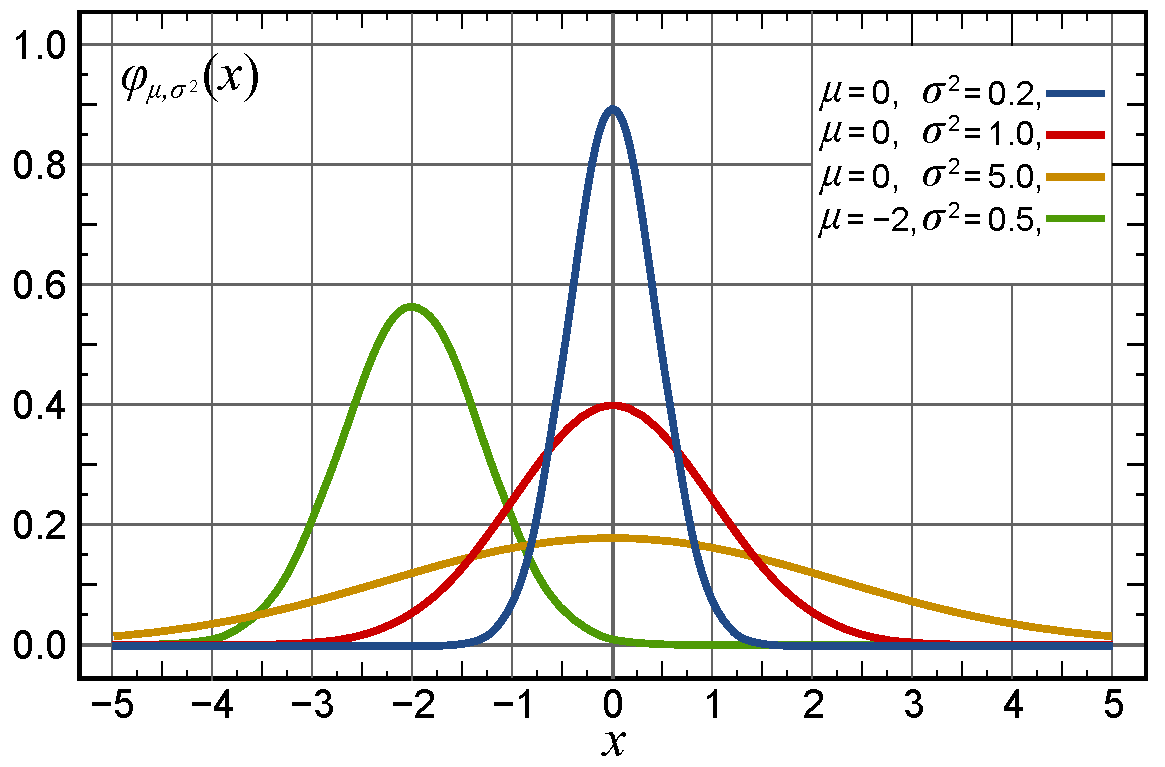
\includegraphics[width = 3.3cm]{./img/normal_pdf.pdf}}
		\parbox{3.3cm}{\emph{KVF/CDF:} \\ 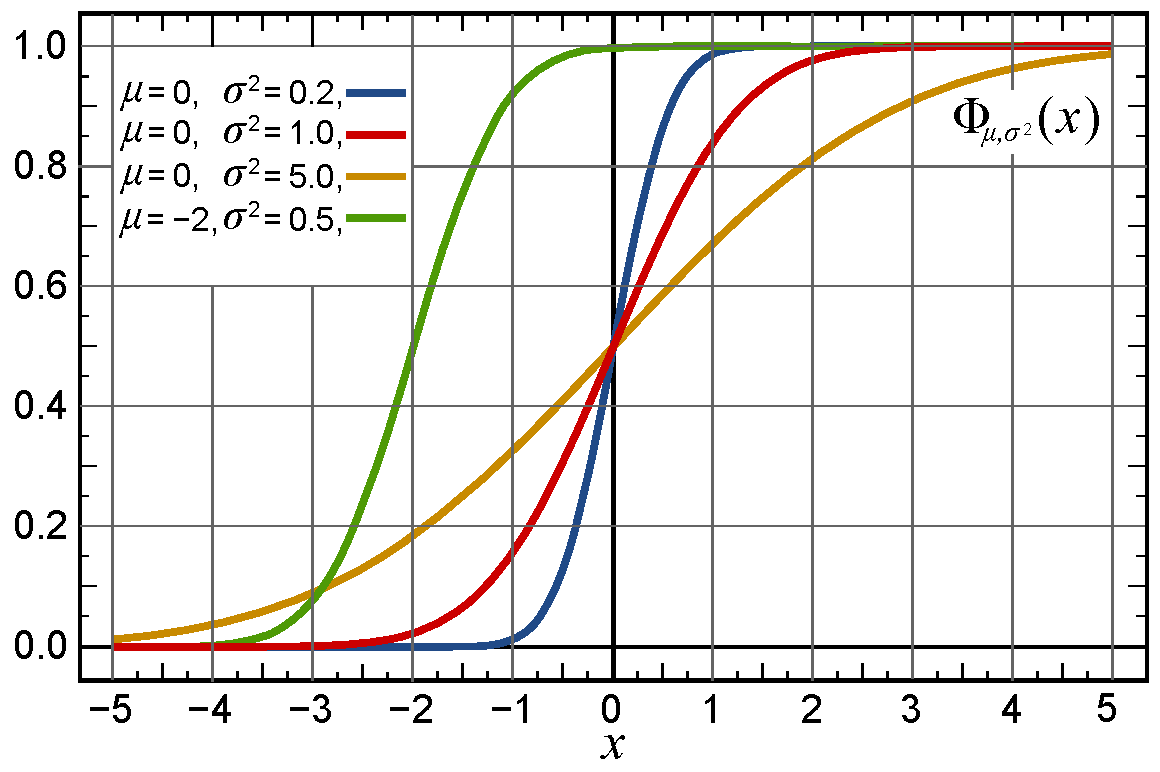
\includegraphics[width = 3.3cm]{./img/normal_cdf.pdf}}
		\textbf{WDF: }
		\boxed{f_X (x) = \frac{1}{\sqrt{2 \pi \sigma^2}} e^{-\frac{(x-\mu)^2}{2 \sigma^2}} \quad x \in \mathbb R} \qquad \parbox{1.2cm}{$\mu \in \mathbb R$ \\[0.5em] $\sigma > 0$}

		\begin{tablebox}{lll}
		\everymath{\displaystyle}
			$\underset{\text{Erwartungswert}}{\E(\X) = \mu}$ & $\underset{\text{Varianz}}{\Var(\X) =\sigma^2}$ & $\underset{\text{Charakt. Funktion}}{\varphi_{\X}(\omega) = e^{j\omega\mu-\frac{\omega^2\sigma^2}{2}}}$\\
		\end{tablebox} \everymath{\textstyle}
\end{sectionbox}

\begin{sectionbox}
	\subsection{Sonstiges}
	\textbf{Gammadistribution} $Γ(α,β)$: $\E[\X] = \frac{α}{β}$\\
	\textbf{Exponential:} $f(x,λ) = λ e^{-λx}$ \quad $\E[\X] = λ^{-1}$ \quad $\Var[\X] = λ^{-2}$
\end{sectionbox}

% Section
% ----------------------------------------------------------------------
\section{Wichtige Parameter}
% ======================================================================
\begin{sectionbox}
	\subsection{Erwartungswert (1. zentrales Moment)}
	gibt den mittleren Wert einer Zufallsvariablen an

	\begin{emphbox}
		$μ_{\X} = \E [\X] = \underset{\text{diskrete} \X:\Omega \ra \Omega'}{\sum\limits_{x \in \Omega'} x \cdot \P_{\X}(x)} \quad \stackrel{\wedge}{=}\quad \underset{\text{stetige} \X: \Omega \ra \R}{\int \limits_{\R} x \cdot f_{\X} (x) \diff x}$
	\end{emphbox}
	$\E[\alpha \X + \beta \Y] = \alpha \E [\X] + \beta \E[\Y]$ \hfill $\X \le \Y \Ra \E[\X] \le \E[\Y]$\\
	$\E[X^2] = \Var[X] + \E[X]^2$ \\
	$\E[\X\Y] = \E[\X] \E[\Y]$, falls $\X$ und $\Y$ stochastisch unabhängig\\
	Umkehrung nicht möglichich: Unkorrelliertheit $\not \Ra$ Stoch. Unabhängig! \\

	\subsubsection{Für Funktionen von Zufallsvariablen $g(x)$}
	$\E[g(\X)] = \sum \limits_{x \in \Omega'} g(x) \P_{\X} (x)\quad \stackrel{\wedge}{=}\quad \int \limits_{\R} g(x) f_X (x) \diff x$

\end{sectionbox}



\begin{sectionbox}
\subsection{Varianz (2. zentrales Moment)}
	ist ein Maß für die Stärke der Abweichung vom Erwartungswert
	\begin{emphbox}
		$σ_{\X}^2 = \Var [X] = \E \big[(\X - \E[\X])^2\big] = \E[\X^2] - \E[\X]^2$
	\end{emphbox}
	$\Var [ \alpha \X + \beta] = \alpha^2 \Var [\X]$ \hfill $\Var [\X] = \Cov [\X,\X]$\\[0.5em]
	$\Var \left[\sum \limits_{i=1}^n \X_i \right] = \sum \limits_{i=1}^{n} \Var [\X_i] + \sum\limits_{j \not= i} \Cov[\X_i, \X_j]$\\
	\textbf{Standard Abweichung:} $\sigma = \sqrt{\Var[\X]}$
\end{sectionbox}

\begin{sectionbox}
\subsection{Kovarianz}
	Maß für den linearen Zusammenhang zweier Variablen
	\begin{emphbox}
		$\Cov [\X,\Y] = \E[(\X- \E[\X])(\Y - \E[\Y])^\top] = $\\[0.5em]
		$ = \E [\X\Y^\top] - \E[\X] \E[\Y]^\top = \Cov[\Y, \X]$
	\end{emphbox}
	$\Cov [\alpha \X + \beta, \gamma \Y + \delta] = \alpha \gamma \Cov [\X, \Y]$ \\
	$\Cov [ \X + \textit U, \Y + \textit V] = \Cov [\X, \Y] + \Cov [\X, \textit V] + \Cov [\textit U, \Y] + \Cov [\textit U, \textit V]$ \\

	\subsubsection{Korrelation = standardisierte Kovarianz}
	$\rho(\X,\Y) = \frac{\Cov[\X,\Y]}{\sqrt{\Var[\X] \cdot \Var[\Y]}} = \frac{C_{x,y}}{σ_x \cdot σ_y}$ \qquad $\rho(\X,\Y) ∈ [-1;1]$

	\subsubsection[Kovarianzmatrix]{Kovarianzmatrix für $\vec z = (\vec x, \vec y)^\top$}
	$\Cov[\vec z] = \ma C_{\vec z} = \mat{C_{\X} & C_{\X\!\Y} \\ C_{\X\!\Y} & C_{\Y}} = \mat{\Cov[\X,\X] & \Cov[\X,\Y] \\ \Cov[\Y,\X] & \Cov[\Y,\Y]}$\\
	Immer symmetrisch: $C_{xy} = C_{yx}$! Für Matrizen: $\ma C_{\vec x \vec y} = \ma C_{\vec y \vec x}^\top$
\end{sectionbox}

% \begin{sectionbox}
% 	\subsection{Schiefe (3. zentrales Moment)}
% 	Maß für die Asymmetrie einer Wahrscheinlichkeitsverteilung.\\
% 	$v(\X) = \E\left[ \left( \frac{\X - \E[\X]}{\sqrt{\Var[\X]}} \right)^3 \right]$ \qquad \parbox{4cm}{$v(\X) < 0$: links schief/flacher \\ $v(\X) > 0$: rechts schief/flacher}
% \end{sectionbox}


% \begin{sectionbox}
% 	\subsection{Momente}
% 	\begin{tablebox}{ll}
% 	Erwartungswert & $\mu_{\X}(n) = E[\X_n]$\\
% 	Varianzfolge & $\sigma^2_{\X}(n) = Var[\X_n] = E[\X_n^2] - E[\X_n]^2$\\
% 	Autokorrelation & $r_{\X}(k,l) = E[\X_k \X_l]$\\
% 	Autokovarianzf. & $c_{\X}(k,l) = Cov[\X_k,\X_l]$ \newline $= r_{\X}(k,l) - \mu_{\X}(k) \mu_{\X}(l)$\\
% 	\end{tablebox}
% \end{sectionbox}


% Section
% ----------------------------------------------------------------------
\section{Estimation}
%

\begin{sectionbox}
	\subsection{Estimation}
	Statistic Estimation treats the problem of inferring underlying characteristics of unknown random
variables on the basis of observations of outputs of those random variables.

	\begin{tablebox}{lll}
		Sample Space $Ω$ & nonempty set of outputs of experiment\\
		Sigma Algebra $\mathbb F \subseteq 2^Ω$ & set of subsets of outputs (events)\\
		Probability $\P: \mathbb F \mapsto [0,1]$ & \\
		Random Variable $\X: Ω \mapsto \mathbb X$ & mapped subsets of $Ω$\\
		Observations: $x_1, \ldots, x_N$ & single values of $\X$\\
		Observation Space $\mathbb X$ & possible observations of $\X$\\
		Unknown parameter $θ ∈ Θ$ & parameter of propability function\\
		Estimator $T: \mathbb X \mapsto Θ$ & $T(\X) = \hat{θ}$, finds $\hat{θ}$ from $\X$\\
	\end{tablebox}

	\begin{symbolbox}
		unknown parm. $θ$ \qquad estimation of param. $\hat{θ}$\\
		R.V. of param. $Θ$ \qquad estim. of R.V. of parm $\textit T(\X) = \hat {Θ}$
	\end{symbolbox}

\end{sectionbox}


\begin{sectionbox}
	\subsection{Quality Properties of Estimators}
	Consistent: If $\lim\limits_{N \ra ∞} T(x_1, \ldots, x_N) = θ$\\
	Bias $\Bias(T) := \E [T(\X_1, \ldots, \X_N)] - θ$ \\
	unbiased if $\Bias(T)=0$ (biased estimators can provide better estimates than unbiased estimators.)\\
	Variance $\Var[T] := \E\left[ (T − \E[T])^2 \right]$
\end{sectionbox}



\begin{sectionbox}
	\subsection{Mean Square Error (MSE)}
	The MSE is an extension of the Variance $\Var[T] := \E\left[ (T − \E[T])^2 \right]$:\\
	\begin{emphbox}
		MSE: $ε[T] = \underset{=\E[(\hat{θ}-θ)^2]}{\E\left[(T − θ)^2\right]} = \Var(T) + (\mathrm{Bias}[T])^2$
	\end{emphbox}
	If $Θ$ is also r.v. $\Ra$ mean over both (e.g. Bayes est.):\\
	\textbf{Mean MSE:} $\E[(T(\X)-Θ)^2] = \E\left[\E\left[(T(\X) − Θ)^2|Θ=θ\right]\right]$

	\subsubsection{Minimum Mean Square Error (MMSE)}
	Minimizes mean square error: $\underset{\hat{θ}}{\arg\min} \E\left[(\hat{θ} − θ)^2\right]$\\
	$\E\left[(\hat{θ} − θ)^2\right] = \E[θ^2] - 2\hat{θ} \E[θ] + \hat{θ}^2$\\
	Solution: $\frac{\diff}{\diff \hat{θ}} \E\left[(\hat{θ} − θ)^2\right] \stackrel{!}{=} 0 = - 2\E[θ] + 2\hat{θ}$\quad$\Ra$ $\hat{θ}_{\ir MMSE}=\E[θ]$

\end{sectionbox}


\begin{sectionbox}
	\subsection{Maximum Likelihood}
	Given model $\{\mathbb X, \mathbb F, \P_θ ; θ ∈ Θ\}$, assume $\P_θ(\vec x)$ or $f_{\vec {\X}}(\vec x,θ)$ for observed data $\vec x$. Estimate parameter $θ$ so that the likelihood $L(\vec x,θ)$ or $L(θ|\X=\vec x)$ to obtain $\vec x$ is maximized.\\
	\\
	\textbf{Likelihood Function:} (Prob. for $θ$ given $\vec x$)\\
	\begin{tabular}{@{}ll}
		Discrete: & $L(x_1, \ldots, x_N; θ) = \P_θ(x_1, \ldots, x_N)$\\
		Continuous: & $L(x_1, \ldots, x_N; θ) = f_{\X_1, ... , \X_N}(x_1, \ldots, x_N, θ)$\\
	\end{tabular}
	%Likelihood functions often in log scale \\
	%Prob. dens. to get $\vec x$ with $θ$ is used as parameter\\
	If $N$ observations are Identically Independently Distributed (i.i.d.):\\
	$L(\vec x, θ) = \prod\limits_{i=1}^N \P_θ(x_i) = \prod\limits_{i=1}^N f_{\X_i}(x_i)$\\
	\\
	\textbf{ML Estimator} (Picks $θ$): $T_{\ir ML} : \X \mapsto \underset{θ ∈ Θ}{\argmax} \{ L(\X,θ) \} = $\\
	$= \underset{θ ∈ Θ}{\argmax} \{ \log L(\vec{\X},θ) \} \stackrel{\text{i.i.d.}}{=} \underset{θ ∈ Θ}{\argmax} \big\{ \sum \log L(x_i,θ) \big\}$\\
	%If known $\vec x$ are fixed, $L$ only depends on $θ$\\
	Find Maximum: $\frac{∂ L(\vec x,θ)}{∂ θ} = \left. \frac{\diff}{\diff θ} \log L(x; θ) \right|_{θ = \hat \theta} \stackrel{!}{=} 0$\\
	Solve for $θ$ to obtain ML estimator function $\hat{θ}_{\ir ML}$\\

		Check quality of estimator with MSE\\
	Maximum-Likelihood Estimator is Asymptotically Efficient. However, there might be not enough samples and the likelihood function is often not known.

\end{sectionbox}



\begin{sectionbox}
	\subsection{Uniformly Minimum Variance Unbiased (UMVU) Estimators (Best unbiased estimators)}
	Best unbiased estimator: Lowest Variance of all estimators.\\
	Fisher’s Information Inequality: Estimate lower bound of variance if
	\begin{itemize}
		\item $L(x,θ) > 0, ∀x,θ$
		\item $L(x,θ)$ is diffable for $θ$
		\item $\int_{\mathbb X} \frac{\partial}{\partial θ} L(x,θ) \diff x = \frac{\partial}{\partial θ} \int_{\mathbb X} L(x,θ) \diff x$\
	\end{itemize}
	\textbf{Score Function:}\\
	$g(x, θ) = \frac{\partial}{\partial θ} \log L(x,θ) = \frac{\frac{\partial}{\partial θ} L(x,θ)}{L(x,θ)}$ \qquad $\E[g(x,θ)] = 0$\\
	\textbf{Fischer Information:} \\
	$I_{\ir F}(θ) := \Var[g(\X,θ)] = \E[g(x,θ)^2] = -\E\left[ \frac{\partial^2}{\partial θ^2} \log L(\X, θ) \right]$\\
	\textbf{Cramér-Rao Lower Bound (CRB):}\quad (if $T$ is unbiased)
	\begin{emphbox}
		$\Var[T(\X)] \ge \left( \frac{\partial \E[T(\X)]}{\partial θ}\right)^2 \frac{1}{I_{\ir F}(θ)}$ \qquad $\Var[T(\X)] \ge \frac{1}{I_{\ir F}(θ)}$
	\end{emphbox}
	For $N$ i.i.d. observations: $I_{\ir F}^{(N)}(x,θ) = N \cdot I_{\ir F}^{(1)}(x,θ)$
	\subsubsection{Exponential Models}
	If $f_{\X}(x) = \frac{h(x)\exp\big(a(θ)t(x)\big)}{\exp(b(θ))}$ then $I_F(θ) = \frac{∂a(θ)}{∂θ} \frac{∂ E[t(\X)]}{∂ θ}$\\
	\\
	\textbf{Some Derivations:} (check in exam)\\
	Uniformly: Not diffable $\Ra$ no $I_F(θ)$\\
	Normal $\mathcal N(θ,σ^2)$: $g(x,θ) = \frac{(x-θ)}{σ^2}$ \quad $I_{\ir F}(θ) = \frac{1}{σ^2}$\\
	Binomial $\mathcal B(θ,K)$: $g(x,θ) = \frac{x}{θ} - \frac{K-x}{1-θ}$ \quad $I_{\ir F}(θ)=\frac{K}{θ(1-θ)}$
\end{sectionbox}


\begin{sectionbox}
	\subsection{Bayes Estimation (Conditional Mean)}
	A Priori information about $θ$ is known as probability $f_Θ(θ; σ)$ with random variable $Θ$ and parameter $σ$.
	Now the conditional pdf $f_{\X|Θ}(x,θ)$ is used to find $θ$ by minimizing the mean MSE instead of uniformly MSE.
	Mean MSE for $Θ$: $\E\left[\E[(\textit T(\X)-Θ)^2|Θ=θ]\right]$

	\textbf{Conditional Mean Estimator:}\\
	$\textit T_{\ir CM}: x \mapsto \E[Θ|\X = x] = \int_{Θ} θ \cdot f_{Θ|\X}(θ|x)\diff θ$\\
	Posterior $f_{Θ|\vec {\X}}(θ|\vec x) = \frac{f_{\vec {\X}|Θ}(\vec x) f_{θ}(θ)}{\int_{Θ} f_{\vec {\X},\xi}(\vec x, ξ) \diff ξ } = \frac{f_{\vec {\X}|θ}(\vec x) f_{θ}(θ)}{f_{\X}(x)}$\\[1em]
	\textbf{Hint:} to calculate $f_{Θ|\vec {\X}}(θ|\vec x)$: Replace every factor not containing $θ$, such as $\frac{1}{f_{\X}(x)}$ with a factor $γ$ and determine $γ$ at the end such that $\int_{Θ} f_{Θ|\vec {\X}}(θ|\vec x) \diff θ = 1$\\
	MMSE: $\E[\Var[\X|Θ=θ]]$\\
	\\
	\textbf{Multivariate Gaussian:} $\X,Θ \sim \mathcal N$ \quad $\Ra σ_{\X}^2 = σ^2_{\X|Θ=θ} + σ_Θ$\\
	$T_{\ir CM}: x \mapsto \E[Θ|\X = x] = \vec{μ}_Θ + \ma C_{Θ,\X} \ma C^{−1}_{\X} (\vec x − \vec {μ}_{\X} )$\\
	MMSE:\\$\E\left[ \norm{T_{\ir CM} − Θ}^2_2 \right] = \operatorname{tr}(\ma C_{θ|\X}) = \operatorname{tr}(\ma C_{Θ} - \ma C_{Θ,\X} \ma C^{−1}_{\X} \ma C_{\X,Θ})$\\
	\\
	\textbf{Orthogonality Principle:}\\
	$T_{\ir CM}(\vec{\X}) − Θ \perp h(\vec \X)$ \quad $\Ra$ \quad  $\E[(\textit T_{\ir CM}(\vec{\X}) − Θ)h(\vec{\X})] = 0$


	\textbf{MMSE Estimator:} $\hat{θ}_{\ir MMSE} = \underset{θ ∈ Θ}{\arg \min}$ MSE\\
	minimizes the MSE for all estimators
\end{sectionbox}



\begin{sectionbox}
	\subsection{Example:}
	Estimate mean $θ$ of $\X$ with prior knowledge $θ ∈ Θ\sim \mathcal N$:\\
	$\X \sim \mathcal N(θ,σ^2_{\X|Θ=θ})$ and $Θ \sim \mathcal N(m, σ^2_Θ)$\\
	$\hat{θ}_{\ir CM} = \E[Θ|\vec{\X} = \vec x] = \frac{N σ^2_Θ}{σ^2_{\X|Θ=θ} + N σ^2_Θ} \hat{θ}_{\ir ML} +\frac{σ^2_{\X|Θ=θ} }{σ^2_{\X|Θ=θ}+N σ^2_Θ} m$\\
	\\
	For $N$ independent observations $x_i$: $\hat{θ}_{\ir ML} = \frac1N \sum x_i$\\
	Large $N \Ra$ ML better, small $N \Ra $ CM better\\
\end{sectionbox}



\columnbreak

% Section
% ----------------------------------------------------------------------
\section{Linear Estimation}
% ========================================================================================
\begin{emphbox}
	$t$ is now the unknown parameter $θ$, we want to estimate $y$ and $\vec x$ is the input vector...  review regression problem $\vec y = \ma A \vec x$ (we solve for $\vec x$), here we solve for $\vec t$, because $\vec x$ is known (measured)! Confusing...\\
	1. Training $\ra$ 2. Estimation\\
	Training: We observe $y$ and $\vec x$ (knowing both) and then based on that we try to estimate $y$ given $\vec x$ (only observe $\vec x$) with a linear model $\hat y=\vec x^\top\vec t$
\end{emphbox}

\begin{sectionbox}
	\begin{emphbox}
		Estimation: $\hat y = \vec x^\top \vec t + m$ \quad or \quad $\hat y = \vec x^\top \vec t$\\
	\end{emphbox}
	Given: $N$ observations $(y_i, \vec x_i)$, unknown parameters $\vec t$, noise $m$\\
	$\vec y = \mat{y_1 \\ \svdots \\ y_n}$ \quad $\ma X = \mat{\vec{x}_1^\top \\ \svdots \\ \vec{x}_n^\top}$ \qquad Note: $\hat y ≠ y$!!\\
	Problem: Estimate $y$ based on given (known) observations $\vec x$ and unknown parameter $\vec t$ with assumed linear Model: $\hat y = \vec x^\top \vec t$\\
	Note $y = \vec x^\top \vec t + m \ra y = \vec x^{'\top} \vec t'$ with $\vec x'=\vect{\vec x \\ 1}$,\quad$t'=\vect{\vec t \\ m}$\\
	\\
	Sometimes in Exams: $\hat y = \vec x^\top \vec t \Leftrightarrow \hat{\vec x} = \ma T^\top \vec y$\\ estimate $\vec x$ given $\vec y$ and unknown $\ma T$\\
\end{sectionbox}

\begin{sectionbox}
	\subsection{Least Square Estimation (LSE)}
	Tries to minimize the square error for linear Model: $\hat y_{\ir LS} = \vec x^\top \vec t_{\ir LS}$\\
	Least Square Error: $\min \left[ \sum\limits_{i=1}^N (y_i - \vec x_i^\top \vec t)^2 \right] = \min\limits_{\vec t} \norm{\vec y - \ma X \vec t}$\\
	\begin{emphbox}
		$\vec t_{\ir LS} = (\ma X^\top \ma X)^{-1} \ma X^\top \vec y$\\
	\end{emphbox}
	$\hat{\vec y}_{\ir LS} = \ma X \vec t_{\ir LS} \in span(X)$

	\textbf{Orthogonality Principle:} $N$ observations $\vec x_i ∈ \R^d$ \\ $\ma Y − \ma X\ma T_{\ir LS} ⊥ \operatorname{span}[\ma X] \Leftrightarrow \ma Y - \ma X \ma T_{\ir LS} ∈ \operatorname{null}[\ma \X^\top]$, thus\\
	$\ma X^\top (\ma Y − \ma X \ma T_{\ir LS} ) = 0$ and if $N > d ∧ \operatorname{rang}[\ma X] = d$:\\ $\ma T_{\ir LS} = (\ma X^\top \ma X)^{-1} \ma X^\top \ma Y$
\end{sectionbox}



\begin{sectionbox}
	\subsection{Linear Minimum Mean Square Estimator (LMMSE)}
	Estimate $y$ with linear estimator $\vec t$, such that $\hat y = \vec t^\top \vec x + m$ \\
	Note: the Model does not need to be linear! The estimator is linear!
	\begin{emphbox}
		$\hat y_{\ir LMMSE} = \underset{t,m}{\arg \min} \E\left[ \norm{\vec y - ( \vec t^\top \vec x+ m)}_2^2 \right]$
	\end{emphbox}
	If Random joint variable $\vec z = \vect{\vec x \\ y}$ with \\ $\vec {μ}_{\vec z} = \vect{\vec{μ}_{\vec x} \\ μ_y}$ and $\ma C_{\vec z} = \mat{\ma C_{\vec x} & \vec c_{\vec xy} \\ c_{y\vec x} & c_y}$ then\\
	LMMSE Estimation of $y$ given $x$ is\\
	$\hat y = μ_y+\vec c_{y\vec x} \ma C_{\vec x}^{-1}(\vec x-\vec{μ}_{\vec x}) = \underbrace{\vec c_{y\vec x} \ma C_{\vec x}^{-1}}_{=\vec t^\top}\vec x - \underbrace{μ_y + \vec c_{y\vec x} \ma C_{\vec x}^{-1}\vec{μ}_{\vec x}}_{= m}$\\
	Minimum MSE: $\E\left[ \norm{\vec y - (\vec x^\top \vec t + m)}_2^2 \right] = c_y - c_{y\vec x} C_{\vec x}^{-1}\vec c_{\vec xy}$\\
	\\
	\textbf{Hint:} First calculate $\hat y$ in general and then set variables according to system equation.\\
	\textbf{Multivariate:} $\hat{\vec y} = \ma T_{\ir LMMSE}^\top \vec x$ \qquad $ \ma T_{\ir LMMSE}^\top = \ma C_{\vy \vx} \ma C_{\vx}^{-1}$\\
	\rule{\columnwidth}{0.5pt}
	\\
	If $\vec \mu_{\vec z} = \vec 0$ then\\
	Estimator $\hat y = \vec c_{y, \vec x} \ma C^{-1}_{\vec x} \vec x$\\
	Minimum MSE: $\E[c_{y,\vec x}] = c_y - \vec t^\top \vec c_{\vec x,y}$
\end{sectionbox}



\begin{sectionbox}
	\subsection{Matched Filter Estimator (MF)}
	For channel $\vec y = \vec hx + \vec v$, Filtered: $\vec t^\top \vec y = \vec t^\top\vec h x + \vec t^\top \vec v$\\
	Find Filter $\vec t^\top$ that maximizes SNR $= \frac{\norm{ \vec h x}} {\norm{\vec v}}$\\
	$\ma t_{\ir MF} = \underset{t}{\max} \left\{ \frac{\E\left[ (\vec t^\top \vec h x)^2 \right] }{\E\left[ (\vec t^\top \vec v)^2 \right] } \right\}$\\
	\\
	In the lecture (estimate $\vec h$):\\
	$\ma T_{\ir MF} = \underset{T}{\max} \left\{ \frac{\left| \E\left[ \hat{\vec h}^H \vec h \right] \right|^2}{\operatorname{tr}\left[ \Var[\ma T \vec n]\right] } \right\}$\\
	$\hat{\vec h}_{\ir MF} = \ma T_{\ir MF} \vec y$ \qquad $\ma T_{\ir MF} \propto \ma C_{\vec h} \ma S^H \ma C^{-1}_{\vec n}$

\end{sectionbox}





\begin{sectionbox}
	\subsection{Example}

	\begin{center}
		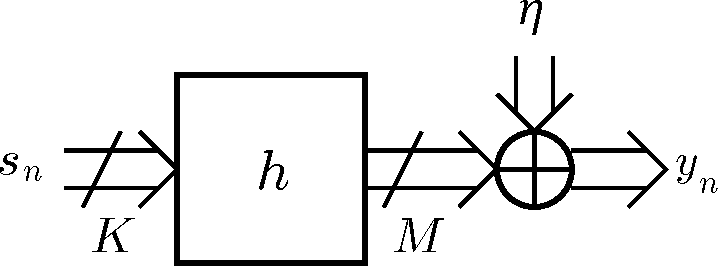
\includegraphics[width = 0.7\columnwidth]{channel}
	\end{center}
	System Model: $\vec y_n = \ma H \vec s_n + η_n$\\
	with $\ma H = (h_{m,k}) \in \C^{M \times K}$ \qquad ($m\in[1,M], k\in[1,K]$)\\
	\textbf{Linear Channel Model} $\vec y = \ma S \vec h + \vec n$ with \\$\vec h \sim \mathcal N (0, \ma C_{\vec h})$ and $\vec n \sim \mathcal N (0, \ma C_{\vec n})$\\
	\\
	Linear Estimator $\ma T$ estimates $\hat {\vec h} = \ma T \vec y \in \C^{MK}$\\
	$\ma T_{\ir MMSE} = \ma C_{\vec h \vec y} \ma C_{\vec y}^{-1} = \ma C_{\vec h} \ma S^{\ir H} (\ma S \ma C_{\vec h} \ma S^{\ir H} + \ma C_{\vec n})^{-1}$\\
	$\ma T_{\ir ML} = \ma T_{\ir Cor} = (\ma S^{\ir H} \ma C^{−1}_{\vec n} \ma S)^{-1} \ma S^{\ir H} \ma C_{\vec n}^{-1}$\\
	$\ma T_{\ir MF} ∝ \ma C_{\vec h} \ma S^{\ir H} \ma C_{\vec n}^{-1}$\\
	For Assumption $\ma S^{\ir H} \ma S = N σ_s^2 \ma 1_{K \times M}$ and $\ma C_{\vec n} = σ_η^2 \ma 1_{N\times M}$\\
	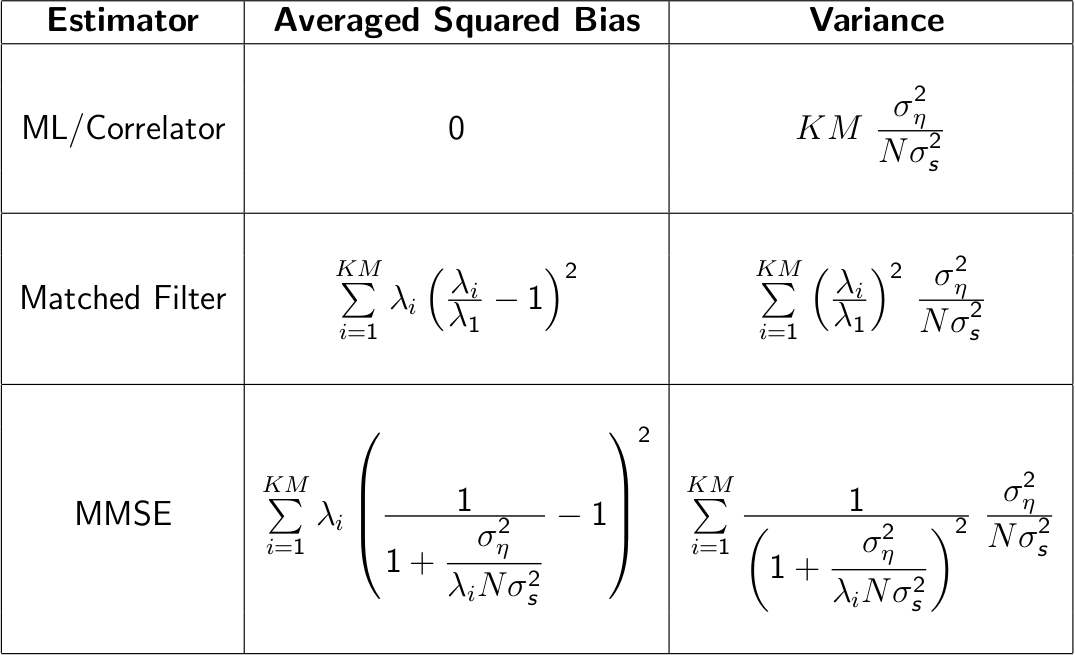
\includegraphics[width = \columnwidth]{comparison}
\end{sectionbox}




\begin{sectionbox}
	\subsection{Estimators}
	Upper Bound: Uniform in $[0;θ]: \hat{θ}_{\ir ML} = \frac{2}{N} \sum x_i$\\
	Probability $p$ for $\mathcal B(p,N)$: $\hat{p}_{\ir ML} = \frac{x}{N}$ \quad $\hat{p}_{\ir CM} = \frac{x+1}{N+2}$\\
	Mean $μ$ for $\mathcal N(μ,σ^2): \hat{μ}^2_{\ir ML} = \frac{1}{N} \sum\limits_{i=1}^N x_i$\\
	Variance $\sigma^2$ for $\mathcal N(μ,σ^2): \hat{σ}^2_{\ir ML} = \frac{1}{N} \sum\limits_{i=1}^N (x_i - μ)^2$

\end{sectionbox}




\vfill

% Section
% ----------------------------------------------------------------------
\section{Gaussian Stuff}

\begin{sectionbox}
	\subsection{Gaussian Channel}
	Channel: $\Y = h s_i + \textit N$ with $h \sim \mathcal N, \textit N \sim \mathcal N$\\
	$L(y_1,...,y_N) = \prod\limits_{i=1}^n f_{\Y_i}(y_i, h)$\\
	$f_{\Y_i}(y_i, h) = \frac{1}{\sqrt{2 \pi} \sigma}\exp\left( - \frac{1}{2 \sigma^2} (y_i - hs_i)^2 \right)$\\
	$\hat h_{ML} = \underset{h}{\operatorname{argmin}} \{\norm{\vec y - h \vec s}^2 \} = \frac{\vec s^\top \vec y}{\vec s^\top \vec s}$\\
	\\
	If multidimensional channel: $\vec y = \ma S \vec h + \vec n$:\\
	$L(\vec y, \vec h) =  \frac{1}{\sqrt{\det(2 \pi \ma C)}}\exp\left( - \frac{1}{2} (\vec y - \ma S \vec h)^\top\ma C^{-1}(\vec y - \ma S \vec h) \right)$\\
	$l(\vec y, \vec h) =  \frac{1}{2} \left( \log(\det(2 \pi \ma C) - (\vec y - \ma S \vec h)^\top\ma C^{-1}(\vec y - \ma S \vec h) \right)$\\
	\\
	$\frac{\diff}{\diff h} (\vec y - \ma S \vec h)^\top\ma C^{-1}(\vec y - \ma S \vec h) = −2 \ma S^\top \ma C^{−1}(\vec y − \ma S\vec h)$


	\textbf{Gaussian Covariance:} if $\Y \sim \mathcal N(0,σ^2), \textit N \sim \mathcal N(0,σ^2)$:\\
	$\ma C_{\Y} = \Cov[\Y,\Y] = \E[(\Y-μ)(\Y-μ)^\top] = \E[\Y\Y^\top]$\\
	For Channel $\Y = S h + \textit N$: $\E[\Y\Y^\top] = S\E[h h^\top]S^\top + \E[\textit N \textit N^\top]$
\end{sectionbox}


\begin{sectionbox}
	\subsection{Multivariate Gaussian Distributions}
	A vector $\vx$ of $n$ independent Gaussian random variables $\x_i$ is jointly Gaussian.
	If $\vx \sim \mathcal N(\vec \mu_{\vx}, \ma C_{\vx})$:\\
	\begin{emphbox}
		$f_{\vx}(\vec x) = f_{\x_1,...,\x_n}(\x_1,...,\x_n) =$ \\[1em] $= \frac{1}{\sqrt{\det(2 π \ma C_{\vx})}} \exp \left( - \frac{1}{2}\left(\vec x - \vec {μ}_{\vx}\right)^\top \ma C_{\vx}^{-1}\left(\vec x - \vec {μ}_{\vx}\right) \right)$\\
	\end{emphbox}

	Affine transformations $\vy = \ma A \vx + \vec b$ are jointly Gaussian with\\
	$\vy \sim \mathcal N(\ma A \vec \mu_{\vx} + \vec b, \ma A \ma C_{\vx} \ma A^\top) $\\
	All marginal PDFs are Gaussian as well

	\textbf{Contour Lines}\\
	Ellipsoid with central point $\E[\vec y]$ and main axis are the eigenvectors of $\ma C_{\vec y}^{-1}$\\

	\subsection{Conditional Gaussian}
	$\VA\!\sim\!\mathcal N(\vec {μ}_{\VA}, \ma C_{\VA}), \VB\!\sim\!\mathcal N(\vec{μ}_{\VB}, \ma C_{\VB})$ \\
		$\Ra (\VA| \VB\!=\!b) \sim \mathcal N(\vec{μ}_{\VA|\VB},\ma C_{\VA|\VB})$\\
	\\
	\textbf{Conditional Mean:}\\
	$\E[\VA|\VB = \vec b] = \vec{μ}_{\VA|\VB=\vec b} = \vec{μ}_{\VA} + \ma C_{\VA\VB}\;\ma C_{\VB\VB}^{-1} \left(\vec b - \vec{μ}_{\VB} \right)$\\
	\\
	\textbf{Conditional Variance:}\\
	$\ma C_{\VA|\VB} = \ma C_{\VA\VA} - \ma C_{\VA\VB}\;\ma C_{\VB\VB}^{-1}\;\ma C_{\VB\VA}$
\end{sectionbox}



\begin{sectionbox}
	\subsection{Misc}
	If CDF of gaussian distribution given $Φ(z) \sim \mathcal N(0,1)$ then for $\X \sim \mathcal N(1,1)$ the CDF is given as $Φ(x - μ_x)$
\end{sectionbox}

% Section
% ----------------------------------------------------------------------
\section{Sequences}
\begin{sectionbox}
	\subsection{Random Sequences}
	Sequence of a random variable. Example: result of a dice is RV, roll a dice several times is a random sequence.

	\subsection{Markov Sequence $X_n : Ω \ra X_n$}
	Sequence of memoryless state transitions with certain probabilities.\\
	1. state: $f_{\X_1}(x_1)$\\
	2. state: $f_{\X_2|\X_1}(x_2|x_1)$\\
	n. state: $f_{\X_n|\X_{n-1}}(x_n|x_{n-1})$\\
\end{sectionbox}



\begin{sectionbox}
	\subsection{Hidden Markov Chains}
	Problem: states $\X_i$ are not visible and can only be guessed indirectly as a random variable $\Y_i$.\\
	\\
	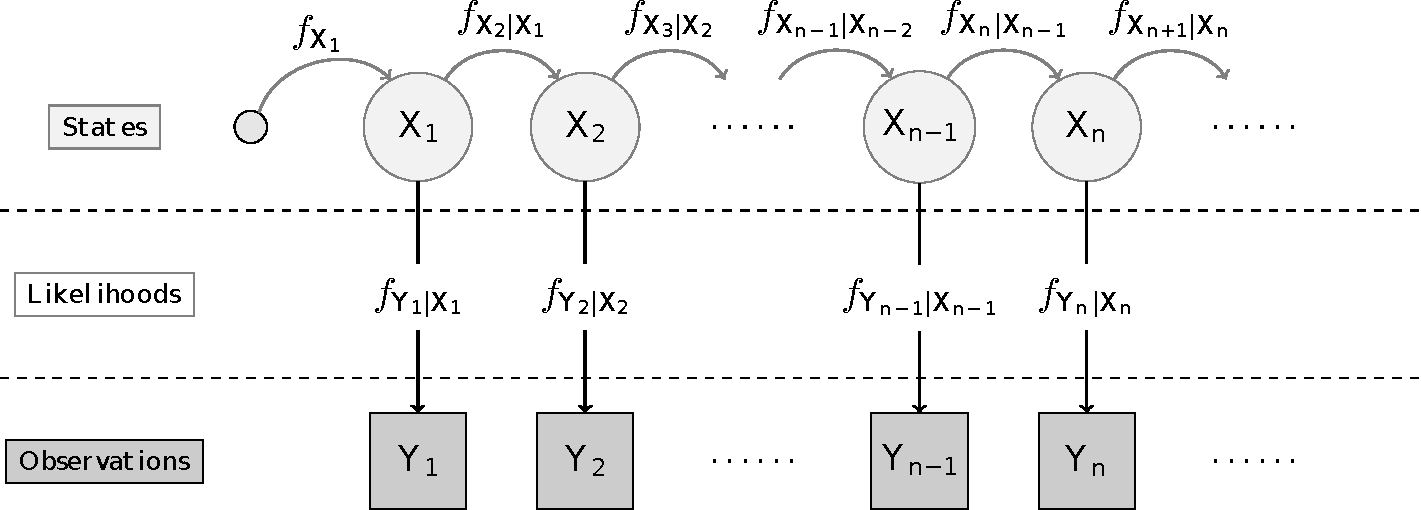
\includegraphics[width=\textwidth]{hidden_markov}

	Conditional pdf $f_{\VX_n|\VY_n}$ \qquad Likelihood pdf $f_{\Y_n|\X_n}$\\
	State-transision pdf $f_{\X_n|\X_{n-1}}$\\
	\textbf{Estimation:}
	\begin{equation*}
		f_{\VX_n|\VY_n} \propto f_{\VY_n|\VX_n} \cdot \int_{\mathbb X} f_{\VX_n|\VX_{n-1}} \cdot f_{\VX_{n-1}|\VY_{n-1}} \diff \vec x_{n-1}
	\end{equation*}
\end{sectionbox}

% Section
% ----------------------------------------------------------------------
\section{Recursive Estimation}

\begin{sectionbox}
	\subsection{Kalman-Filter}
	recursively calculates the most likely state from previous state estimates and current observation. Shows
	optimum performance for Gauss-Markov Sequences.\\

	\textbf{State space:}\\
	$\vec x_n = \ma G_n \vec x_{n−1} + \ma B \vec u_n + \vec v_n$\\
	$\vec y_n = \ma H_n \vec x_{n} + \vec w_n$\\
	\\
	With gaussian process/measurement noise $\vec v_n/\vec w_n$\\
	Short notation: $\E[\vec x_n|\vec y_{n-1}] = \hat {\vec x}_{n|n-1}$ \quad $\E[\vec x_n|\vec y_{n}] = \hat {\vec x}_{n|n}$\\
	$\E[\vec y_n|\vec y_{n-1}] = \hat {\vec y}_{n|n-1}$ \quad $\E[\vec y_n|\vec y_{n}] = \hat {\vec y}_{n|n}$\\
	\\
	\textbf{1. step: Prediction}\\
	Mean: $\hat {\vec x}_{n|n-1} = \ma G_n \hat{\vec x}_{n-1|n-1}$\\
	Covariance: $\ma C_{\vec x_{n|n-1}} = \ma G_n \ma C_{\vec x_{n-1|n-1}} \ma G_n^\top + \ma C_{\vec v}$\\
	\\
	\textbf{2. step: Update}\\
	Mean: $\hat{\vec x}_{n|n} = \hat{\vec x}_{n|n-1} + \ma K_n \left( \vec y_n - \ma H_{n} \hat{\vec x}_{n|n-1} \right)$\\
	Covariance: $\ma C_{\vec x_{n|n}} = \ma C_{\vec x_{n|n-1}} + \ma K_n \ma H_{n} \ma C_{\vec x_{n|n-1}}$\\


	$\hat{\vec x}_{n|n} = \underbrace{\hat{\vec x}_{n|n-1}}_{\hspace{-3em}{\text{estimation} \E[\X_n|\Y_{n-1} = y_{n-1} ]}} + \overbrace{ \ma K_n \underbrace{ \left( \vec y_n - \ma H_{n} \hat{\vec x}_{n|n-1} \right)}_{\text{innovation:} Δy_n}  }^{\text{correction:}\\ \E[\X_n|Δ\Y_n = y_n]}$\\[1em]
	\\
	With optimal \textbf{Kalman-gain} (prediction for $\vec x_n$ based on $\Delta y_n$): \\
	$\ma K_n = \ma C_{\vec x_{n|n-1}} \ma H_{n}^\top ( \underbrace{\ma H_{n} \ma C_{\vec x_{n|n-1}} \ma H_{n}^\top + \ma C_{\vec w_{n}}}_{\ma C_{\delta y_n}})^{-1}$\\
	\\
	\textbf{Innovation}: closeness of the estimated mean value to the real value\\
	$\Delta \vec y_n = \vec y_n - \hat{\vec y}_{n|n-1} =\vec y_n - \ma H_{n} \hat{\vec x}_{n|n-1}$\\
	\\
	\textbf{Init:} $\hat {\vec x}_{0|-1} = \E[\X_0] \qquad σ^2_{0|-1} = \Var[\X_0]$
	\\
	\textbf{MMSE Estimator:} $\hat{\vec x} = \int \vec x_n f_{\X_n | \Y_{(n)}} (\vec x_n | \vec y_{(n)}) \diff \vec x_n$\\
\end{sectionbox}


\begin{sectionbox}
	For non linear problems: Suboptimum nonlinear Filters: Extended KF, Unscented KF, ParticleFilter
	\subsection{Extended Kalman (EKF)}
	Linear approximation of non-linear $g, h$\\
	$\vec x_n = g_n(\vec x_{n−1}, \vec v_n)$ \qquad $\vec v_n \sim \mathcal N$\\
	$\vec y_n = h_n(\vec x_{n−1}, \vec w_n)$ \qquad $\vec w_n \sim \mathcal N$\\

	\subsection{Unscented Kalman (UKF)}
	Approximation of desired PDF $f_{\X_n\!|\!\Y_n}(x_n|y_n)$ by Gaussian PDF.


\end{sectionbox}


\begin{sectionbox}
	\subsection{Particle-Filter}
	For non linear state space \emph{and} non-gaussian noise

	\textbf{Non-linear State space:}\\
	$\vec x_n = g_n(\vec x_{n−1}, \vec v_n)$\\
	$\vec y_n = h_n(\vec x_{n−1}, \vec w_n)$\\


	\textbf{Posterior Conditional PDF:} $f_{\X_n\!|\!\Y_n}(x_n|y_n) \propto \overbrace{ f_{\Y_n\!|\!\X_n}(y_n|x_n) }^{\text{likelihood}} \cdot$\\
	${ \displaystyle \cdot \int\limits_{\mathbb X} \underbrace{ f_{\X_n\!|\!\X_{n-1}}(x_n|x_{n-1}) }_{\text{state transition}} \underbrace{ f_{\X_{n-1}\!|\!\Y_{n-1}}(x_{n-1}|y_{n-1}) }_{\text{last conditional PDF}} \diff x_{n-1} }$


	$N$ random Particles with particle weight $w_n^i$ at time $n$\\
	\textbf{Monte-Carlo-Integration:}
	$I = \E[g(\X)] \approx I_N = \frac{1}{N} \sum\limits_{i=1}^{N} \tilde g(x^i)$\\
	\textbf{Importance Sampling:} Instead of $f_{\X}(x)$ use \textbf{Importance Density} $q_{\X}(x)$\\
	$I_N = \frac{1}{N} \sum\limits_{i=1}^{N} \tilde w^i g(x^i)$ with weights $\tilde w^i = \frac{f_{\X}(x^i)}{q_{\X}(x^i)}$\\
	If $\int f_{\X_n}(x) \diff x \ne 1$ then $I_N = \sum\limits_{i=1}^{N} \tilde w^i g(x^i)$\\
\end{sectionbox}

\begin{sectionbox}
	\subsection{Conditional Stochastical Independence}
	$\P(A \cap B | E) = \P(A | E) \cdot \P(B | E)$\\
	\\
	Given $\Y$, $\X$ and $\Z$ are independent if\\
	$f_{\Z|\Y,\X} (z | y, x) = f_{\Z|\Y}(z|y)$ or\\
	$f_{\X,\Z|\Y} (x,z|y) = f_{\Z|\Y}(z|y) \cdot f_{\X|\Y}(x|y)$\\
	$f_{\Z|\X,\Y}(z|x,y) = f_{\Z|\Y}(z|y)$ or $f_{\X|\Z,\Y}(x|z,y) = f_{\X|\Y}(x|y)$



\end{sectionbox}


% Section
% ----------------------------------------------------------------------
\section{Hypothesis Testing}
making a decision based on the observations

\begin{sectionbox}
	\subsection{Definition}

	Null hypothesis $H_0: θ ∈ Θ_0$ (Assumed first to be true)\\
	Alternate hypothesis $H_1: θ ∈ Θ_1$ (The one to proof) \\
	Descision rule $φ: \mathbb X \ra [0, 1]$ with \\
	$φ(x) = 1$: decide for $H_1$, $φ(x) = 0$: decide for $H_0$
	Error level $α$ with $\E[d(\X)|θ] \le α, ∀θ∈Θ_0$

	\begin{tablebox}{p{7mm}llp{17mm}}
		Error Type & ${}_{\text{Decision}}$\!{\large $\diagdown$}\!${}^{\text{Reality}}$ & $H_1$ false {\small ($H_0$ true)} & $H_1$ true {\small ($H_0$ false)}
		\\ \cmrule
		1 (FA) False& $H_1$ rejected & \textbf{T}rue \textbf{N}egative & \textbf{F}alse \textbf{N}egative (Type 2)
		\\
		Alarm & \small ($H_0$ accepted) & $\P = 1-α$  & $\P = β$
		\\[1em]
		2 (DE) & $H_1$ accepted & \textbf{F}alse \textbf{P}ositive (Type 1) & \textbf{T}rue \textbf{P}ositive
		\\
		Detection Error & \small($H_0$ rejected) & $\P = α$ & $\P = 1-β$
	\end{tablebox}
	Power:
	Sensitivity/Recall/Hit Rate: $\frac{\text{TP}}{\text{TP}+\text{FN}}=1-β$\\
	Specificity/True negative rate: $\frac{\text{TN}}{\text{FP}+\text{TN}}=1-α$\\
	Precision/Positive Prediciton rate: $\frac{\text{TP}}{\text{TP}+\text{FP}}$\\
	Accuracy: $\frac{\text{TP} + \text{TN}}{\text{P}+\text{N}} = \frac{2-α-β}{2}$


	\subsubsection{Design of a test}
	Cost criterion $G_{φ}: Θ \ra [0, 1], θ \mapsto \E[d(X)|θ]$\\
	False Positive lower than $α$: $G_d(θ)|_{θ∈Θ_0} ≤ α, ∀ θ ∈ Θ_0$\\
	False Negative small as possible: $\max \{G_d(θ)|_{θ∈Θ_1}\}, ∀ θ ∈ Θ_1$
\end{sectionbox}



\begin{sectionbox}
	\subsection{Sufficient Statistics}
	Sufficiency for a test $T(\X)$ means that no other test statistic, i.e., function of the observations $\vec x$,
contains additional information about the parameter $θ$ to be estimated:\\
$f_{\X|T} (x|T(x) = t, θ) = f_{\X|T}(x|T (x) = t)$

\end{sectionbox}


% Section
% ----------------------------------------------------------------------
\section{Tests}

\begin{sectionbox}
	\subsection{Neyman-Pearson-Test}
	The best test of $\P_0$ against $\P_1$ is\\
	\parbox{15em}{$d_{\ir NP}(x) = \begin{cases} 1 & R(x) > c\\ γ & R(x) = c \\ 0 & R(x) < c \end{cases}$} \quad \parbox{15em}{ Likelihood-Ratio: \\ $R(x) = \frac{f_{\X}(x; θ_1)}{f_{\X}(x; θ_0)}$ }\\
	$γ = \frac{α - \P_0(\{R > c\})}{\P_0(\{R = c\})}$ \quad Errorlevel $α$\\
	Steps: For $α$ calculate $x_{α}$, then $c = R(x_{α})$\\
	\\
	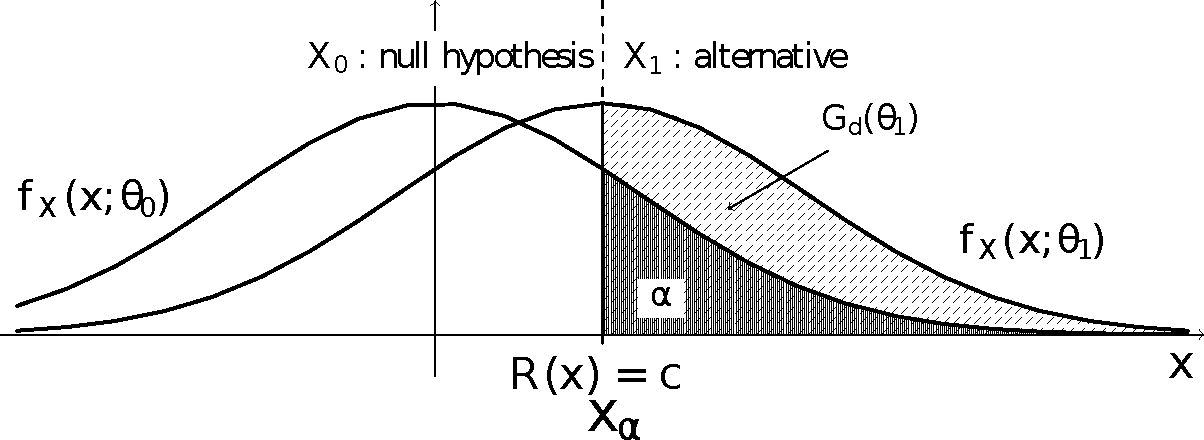
\includegraphics[width = 0.9\columnwidth]{tests}

	\textbf{Maximum Likelihood Detector:} \quad
	$d_{\ir ML}(x) = \begin{cases} 1 & R(x) > 1 \\ 0 & \text{otherwise} \end{cases}$\\
	\textbf{ROC Graphs:} plot $G_d(θ_1)$ as a function of $G_d(θ_0)$
\end{sectionbox}


\begin{sectionbox}
	\subsection{Bayes Test (MAP Detector)}
	Prior knowledge on possible hypotheses: $\P(\{θ ∈ Θ_0 \}) + \P(\{θ ∈ Θ_1\}) = 1$, minimizes the probability of a wrong
decision.\\
	$d_{\ir Bayes} =\! \begin{cases} 1& \!\frac{f_{\X}(x|θ_1)}{f_{\X}(x|θ_0)} > \frac{c_0 \P(θ_0|x)}{c_1 \P(θ_1|x)}\\ 0 & \text{otherwise} \end{cases}$
	$=\! \begin{cases} 1&\!\! \P(θ_1|x) > \P(θ_0|x) \\ 0 &\!\! \text{otherwise} \end{cases}$
	Risk weights $c_0,c_1$ are 1 by default.\\
	If $\P(θ_0) = \P(θ_1)$, the Bayes test is equivalent to the ML test\\
	\textbf{Loss Function} $L(d(x), θ) = \begin{cases} c_0 & \text{type 1 } d(x) = 1, \text{ but }θ = θ_0 \\ c_1 & \text{type 2 } d(x) = 0, \text{ but }θ = θ_1 \end{cases}$
	$\operatorname{risk}(d) = \E[L(d(\X), θ)] = \E [\E [L(d(x), θ)|x = \X ]]$\\
	\textbf{Multiple Hypothesis}
	$d_{\ir Bayes} = \begin{cases} 0 & x ∈ \mathbb X_0 \\ 1 & x ∈ \mathbb X_1 \\ 2 & x ∈ \mathbb X_2 \end{cases}$
\end{sectionbox}


\begin{sectionbox}
	\subsection{Linear Alternative Tests}
	$d: \mathbb X \ra \R, \vec x \mapsto \begin{cases} 1 & \vec w^\top \vec x - w_0 > 0 \\ 0 & \text{otherwise}\end{cases}$\\
	Estimate normal vector $\vec w^\top$, which separates $\mathbb X$ into $\mathbb X_0$ and $\mathbb X_1$\\
	$\log R(\vec x) = \frac{\ln(\det(\ma C_0))}{\ln(\det(\ma C_1))} + \frac{1}{2}(\vec x- \vec{μ}_0)^\top\ma C_0^{-1}(\vec x- \vec{μ}_0) -$ \\ $-\frac{1}{2}(\vec x- \vec{μ}_1)^\top\ma C_1^{-1}(\vec x- \vec{μ}_1) = 0$\\
	\textbf{For 2 Gaussians}, with $\ma C_0 = \ma C_1= \ma C$: $\vec w^\top = (\vec {μ}_1 - \vec{μ}_0)^\top \ma C$\\
	and constant translation $w_0 = \frac{(\vec {μ}_1 - \vec{μ}_0)^\top \ma C (\vec {μ}_1 - \vec{μ}_0)}{2}$\\


	% Bild aus Part7 p 197!!!
	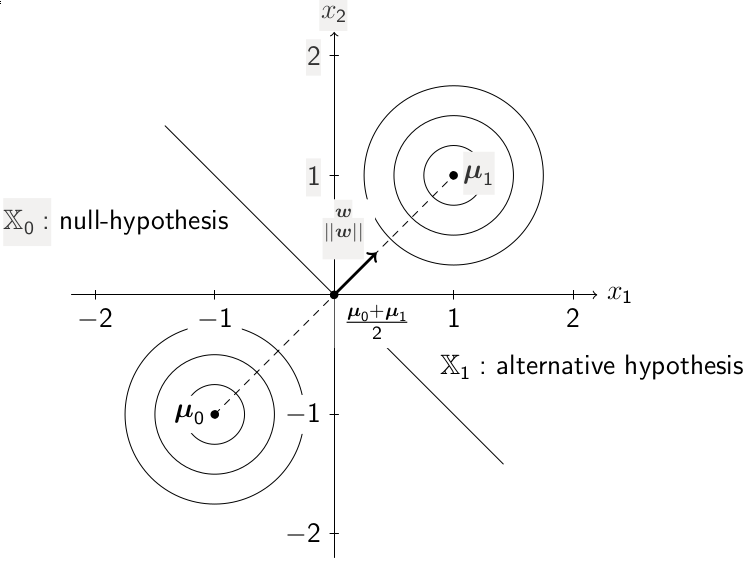
\includegraphics[width = 0.9\columnwidth]{linest2}
\end{sectionbox}







% ======================================================================
% End
% ======================================================================
\end{document}
